\hypertarget{Edge Intelligence}{%
	\chapter{Edge Intelligence}\label{ch:edgeintelligence}}
\thispagestyle{fancy}


Section \ref{sec:ei-background} explains the background for \acrlong{ei}. Section \ref{sec:ei-architecture} describes different edge-centric architectures for \gls{dnn} inference. Section \ref{sec:ei-fast-inference} present enabling technologies for fast inference.


\section{Background}\label{sec:ei-background}

\acrlong{ei} is artificial intelligence applications and services deployed at the edge of the network. The primary objective of \gls{ei} is to enable \gls{ai} for mobile and \gls{iot} application. Progress within \gls{ml} have been pushed by the achievements within \gls{cv} and \gls{nlp} using \gls{dnn}s. However deployment of \gls{dnn} in real applications have been limited to the cloud, as state-of-the-art \gls{dnn} have been too computationally expensive to run elsewhere. The improvement have mostly been impacted by efforts in training deeper models with the ability to learn increasingly complex features. The tendency is exemplified by the winner of ImageNet Challenge \cite{russakovsky_imagenet_2015}; within a time span of only four years, have the number of layers have grown from 8 to 152 layers. 

Proposals of increasingly deeper model have hindered deployment of intelligent services onto mobile and \gls{iot} devices, which have made \gls{ci} inevitable. Running algorithm in large-scale data centers comes with the side-effect of introducing unpredictable communication delays, caused by possibility of congestion in shared communication medium and shared computing resources in the data center. The additional delay from \gls{ci} have made real-time \gls{ai} impractical for mobile and \gls{iot} devices. 
More lightweight, albeit less accurate \gls{dnn} architectures have been proposed to enable \gls{di}, as end-devices have become more powerful in recent years. \gls{ei} is a compromise, which enables deployment of very deep and demanding state-of-the-art \gls{dnn}s on edge server to reduce inference latency, energy consumption and memory footprint of on-device inference, by offloading the heavy task from the end-device onto edge servers, without introducing the communication latency bottleneck by running extremely deep models in the cloud. 

Edge intelligence is a promising compromise to obtain state-of-the-art performance in real-time, necessary for applications such as \gls{ar}/\gls{vr}, \gls{av} and Personal Assistant with very stringent latency and reliability requirements. In edge computing, data processing is done in closer proximity to end-users. The shortened communication path leads to a reduction in communication latency. Edge computing seeks to distibute computing resources, in sharp contrast to the last decade of centralization of computing resources for cloud computing \cite{shi_edge_2016}. Edge computing is envisioned to reliably serve the ever growing number of billions upon billions of connected mobile and \gls{iot} devices. By 2020 Cisco Internet Business Solutions Group, 50 billion things is predicted to be connected to the internet. The amount of data generated by mobile and \gls{iot} device at the edge of the network is expected to overwhelm cloud data centers and exhaust available bandwidth. Hence edge computing is a possible and probably a necessary step in the development and democratizing of \gls{ai}.

Research have shown, that the conventional cloud-only approach in many cases is actually slower than a mobile-only execution in \cite{kang_neurosurgeon:_2017}, as mobile devices are getting more resourceful and nowadays it is not uncommon to have a smartphone equipped with a \gls{gpu}. To avoid draining the battery \gls{iot} devices, it may not be desired to run heavy \gls{ai} algorithms, which makes remote offloading a necessity.  In \cite{karlsen_prototyping_nodate} edge-based offloading are investigated and show significant latency improvement compared to both device- and cloud intelligence by offloading \gls{ai} tasks from \gls{cpu}-enabled end devices to a \gls{gpu}-enabled edge server. 

Furthermore a major concern of cloud computing is privacy. Data generated by end devices might be confidential, hence not allowed to be processed by a data center unless confidentiality can be guaranteed.  Edge computing can may address this concern, as no data is expected to leave the network, as all processing is done at the network edge. However, edge processing alone, does not ensure privacy, as data may be susceptible to interception, as it may be well understood by an adversary. In section \ref{sec:ei-architecture}, it is described how certain edge-centric architectures can promote privacy. 

(Maybe add the push and pull factors of \cite{zhou_edge_2019}) 
 
The survey \citetitle{zhou_edge_2019} by \citet{zhou_edge_2019} review the current state within the research field of \gls{ei}. The survey includes training and inference of \gls{dnn} on the edge and categorizes several performance metrics for \gls{ei} applications and services. This thesis mainly focuses on the inference for real-time application and services and will not address edge-specific training methods. 

In these next section edge-centric architectures for \gls{dnn} model inference.

\newpage
\section{Edge-centric Architectures} \label{sec:ei-architecture}

Figure \ref{fig:edge_arch} illustrates four \gls{dnn} inference architectures at the edge. Using either standalone device  \protect\subref{fig:device-based} or standalone edge \protect\subref{fig:edge-based} is a binary decision, involving whether to process it locally on device or offload the inference task to the edge. Collaborative edge\protect\subref{fig:edge-device-mode} and collaborative edge-cloud \protect\subref{fig:edge-cloud-mode} are both methods were the processing is not done solely by one peer, but a decision is made to offload some of the inference task.
\begin{figure}
	\begin{minipage}{0.65\linewidth}
		\textbf{\protect\subref{fig:device-based} \textsc{Standalone Device}}
		\color{caption-color} \newline
		The end device acquires input data and performs model inference. Since all computation is done on the end device, the performance is solely reliant on the computing resources of the end device. This is also called \acrlong{di}.
	\end{minipage}%
	\hfill
	\begin{minipage}{0.3\linewidth}
		\centering
		\captionsetup[subfigure]{justification=centering}
		\begin{figure}
			\centering
			\subfloat[Device-based\label{fig:device-based}]{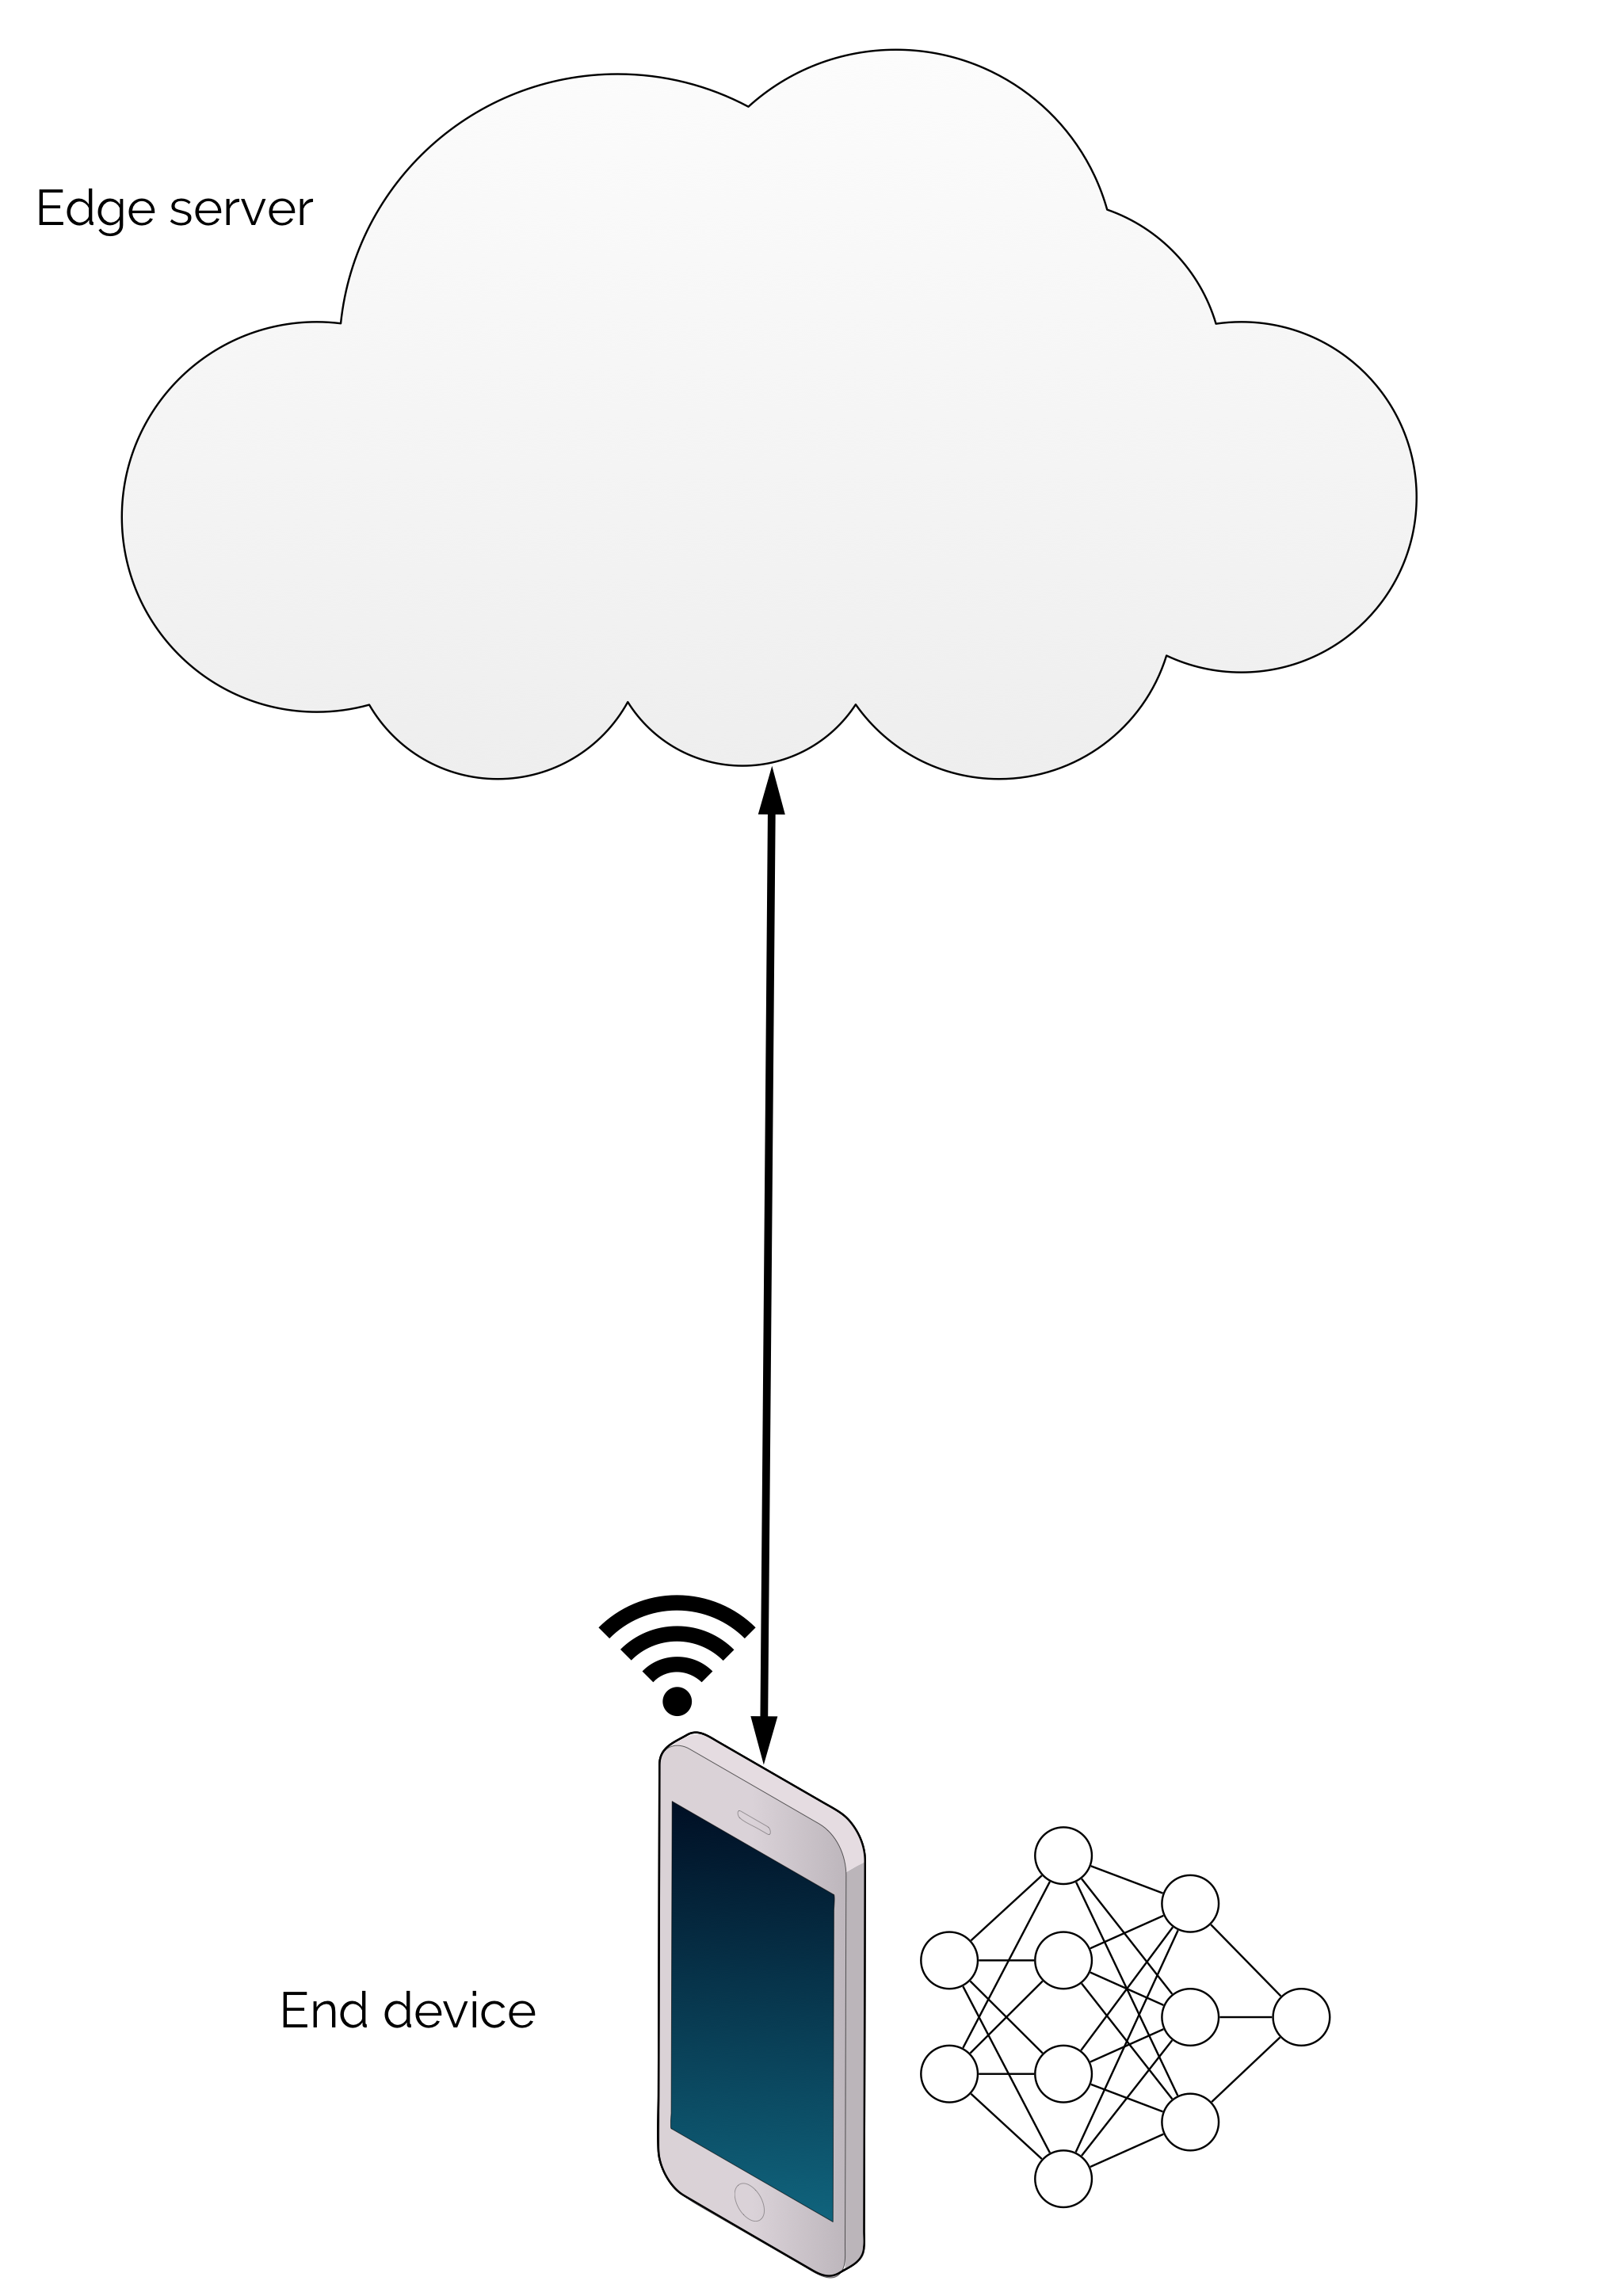
\includegraphics[width=\linewidth]{figures/models/device}}
		\end{figure}
	\end{minipage}
	
	\begin{minipage}{0.3\linewidth}
		\centering
		\begin{figure}
			\centering
			\captionsetup[subfigure]{justification=centering}
			\subfloat[Standalone Edge\label{fig:edge-based}]{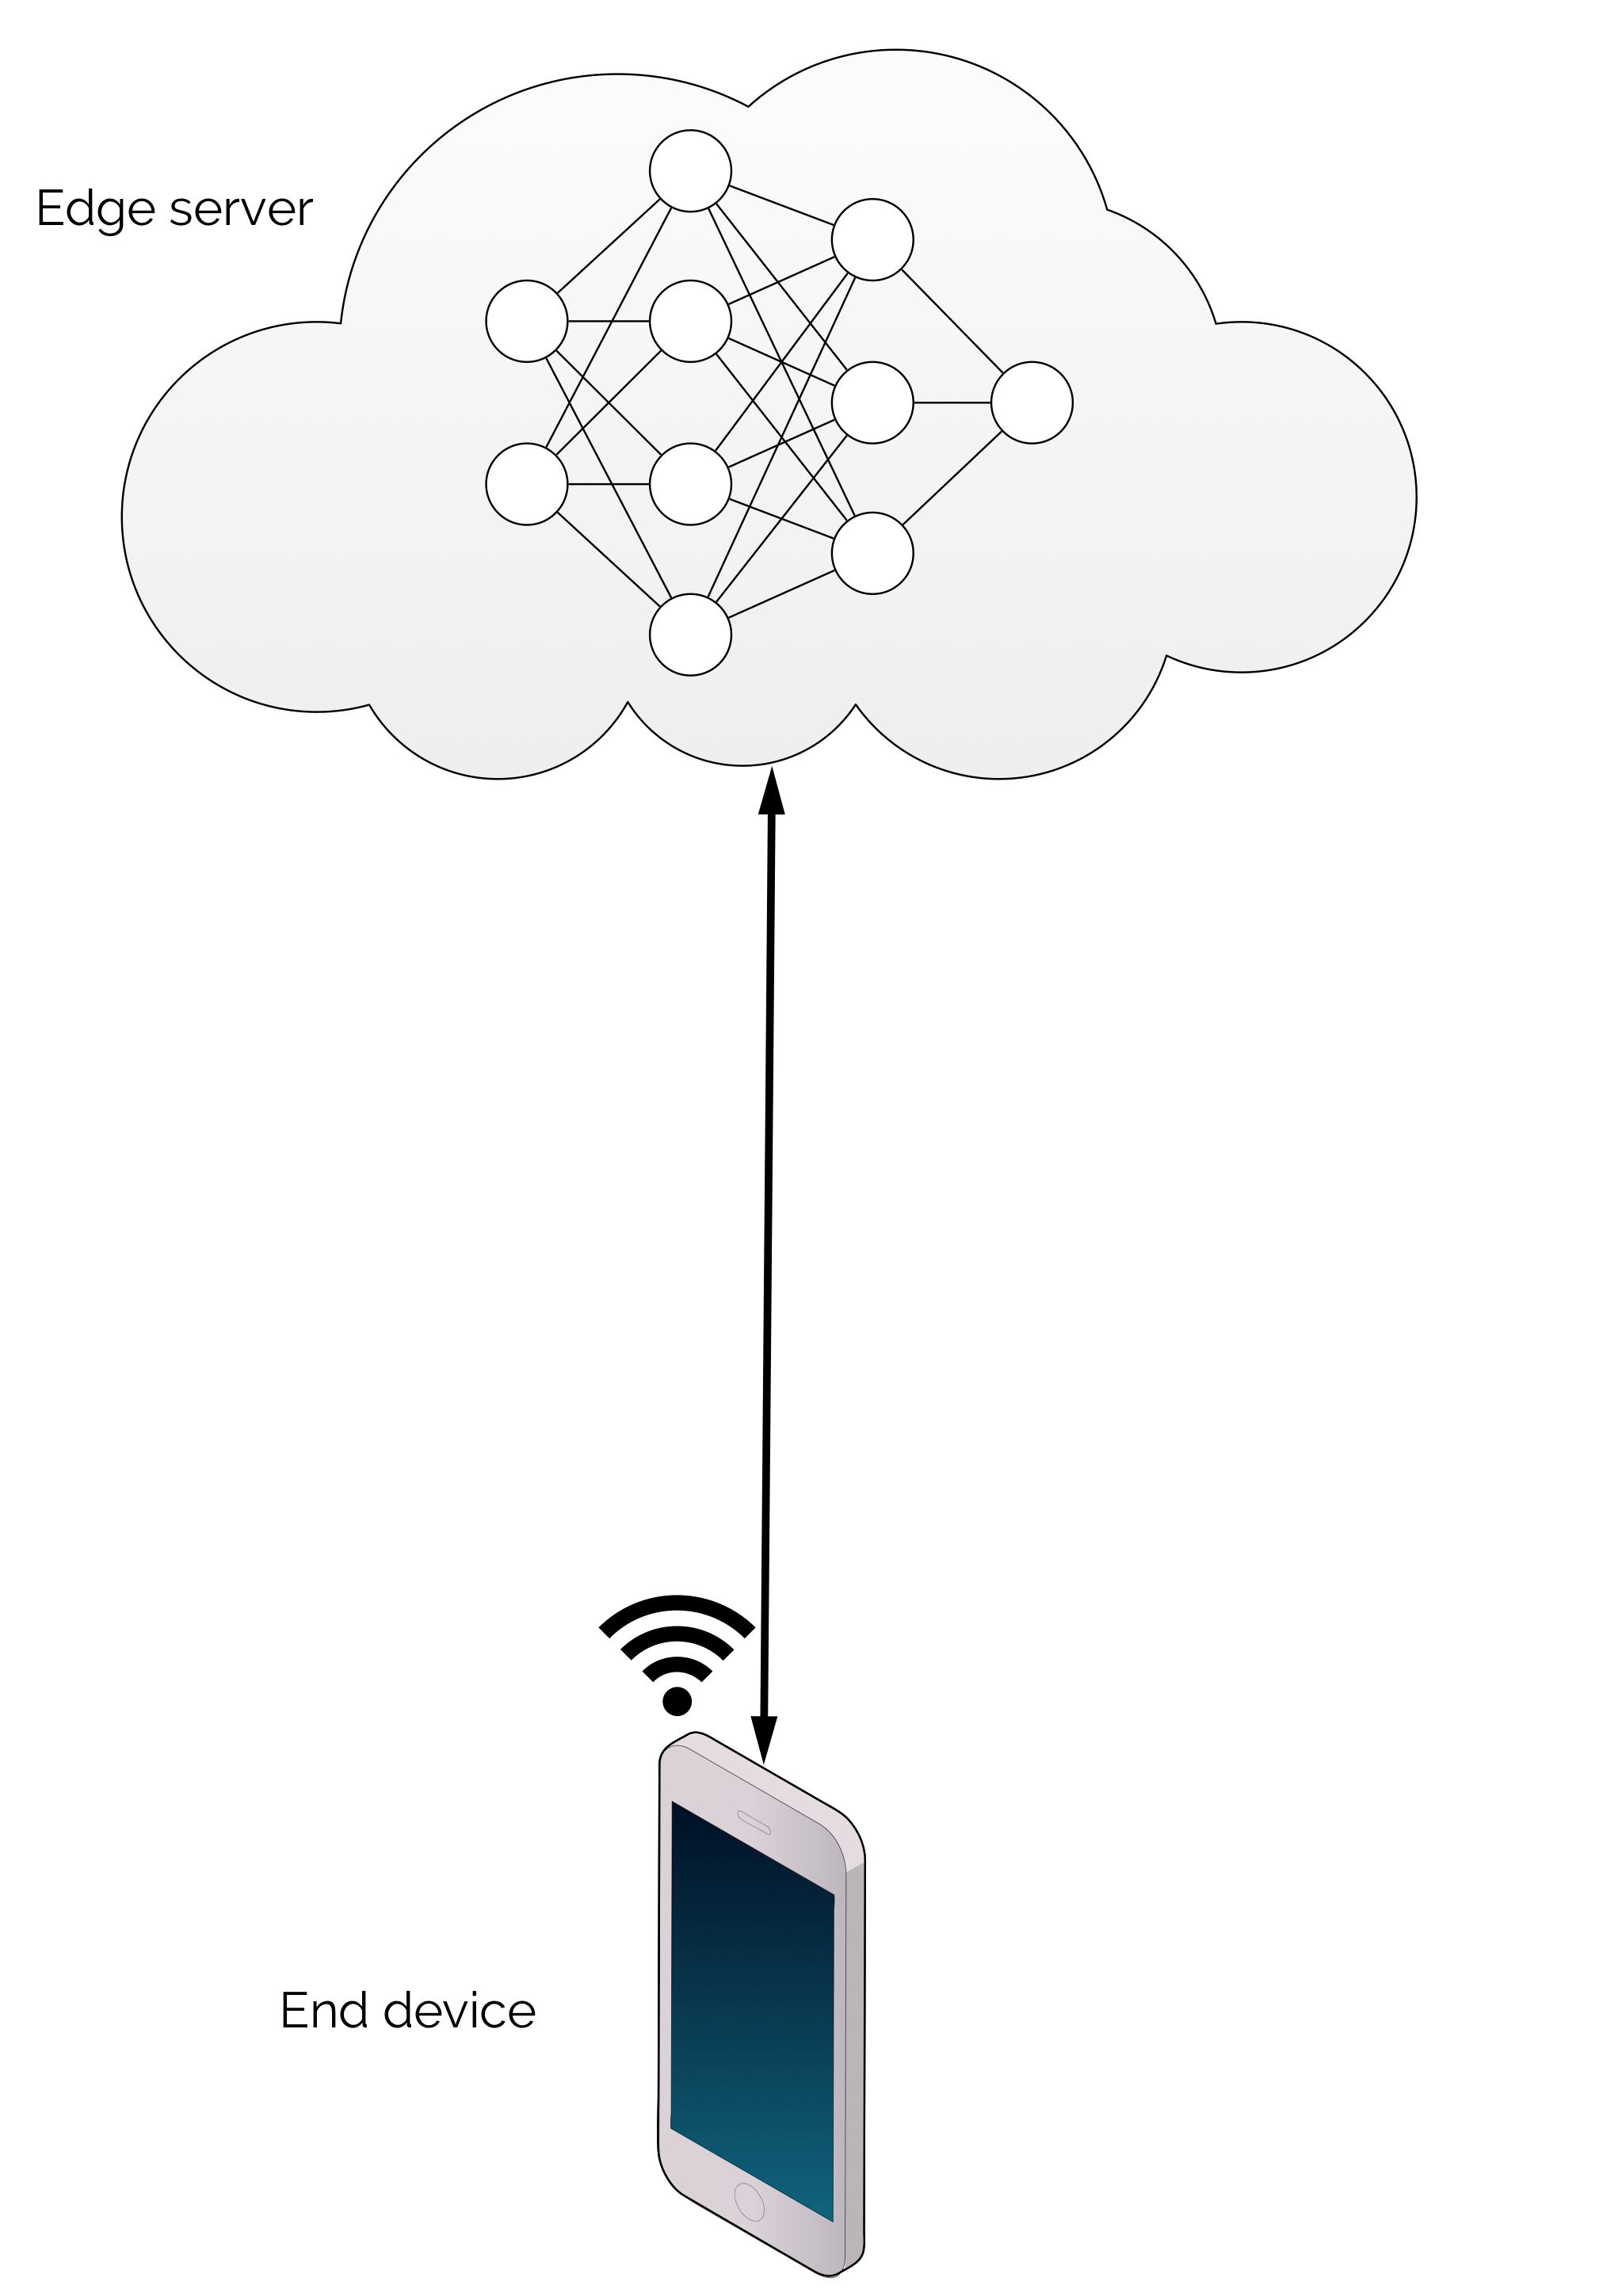
\includegraphics[width=\linewidth]{figures/models/edge}}
		\end{figure}
	\end{minipage}
	\hfill
	\begin{minipage}{0.65\linewidth}
		\textbf{\protect\subref{fig:edge-based} \textsc{Standalone Edge}}
		\color{caption-color} \newline
		Data and model inference is offloaded to the edge. The end device still acquires input data and transfer it to the edge. The edge performs model inference and send back the prediction results to the end device. The performance now relies on edge server computing resources and the available network bandwidth between end device and edge server. If time is the main concern, remote offloading is only sensible, whenever time could be saved, compared to device-based model inference. Or if energy efficiency is the main concern, remote offloading is only sensible if energy could be saved by communicating the data to the edge compared to device-based model inference.
	\end{minipage}
\end{figure}

\begin{figure}
	\begin{minipage}{0.65\linewidth}
		\textbf{\protect\subref{fig:edge-device-mode} \textsc{Collaborative Edge}}
		\color{caption-color} \newline
		The end device acquires input data and performs partially model inference. The intermediate data is transferred to an edge server which finalizes model inference. The performance relies on the computing resource of both the end device and the edge server and edge server workload, as well as available network bandwidth between end device and edge server. Collaborative egde promotes privacy, as intermediate data of model inference is offloaded. These features have no apparent meaning for humans, which will improve the confidentiality of data.   
	\end{minipage}%
	\hfill
	\begin{minipage}{0.3\linewidth}
		\centering
		\captionsetup[subfigure]{justification=centering}
		\begin{figure}
			\centering
			\subfloat[Collaborative Edge\label{fig:edge-device-mode}]{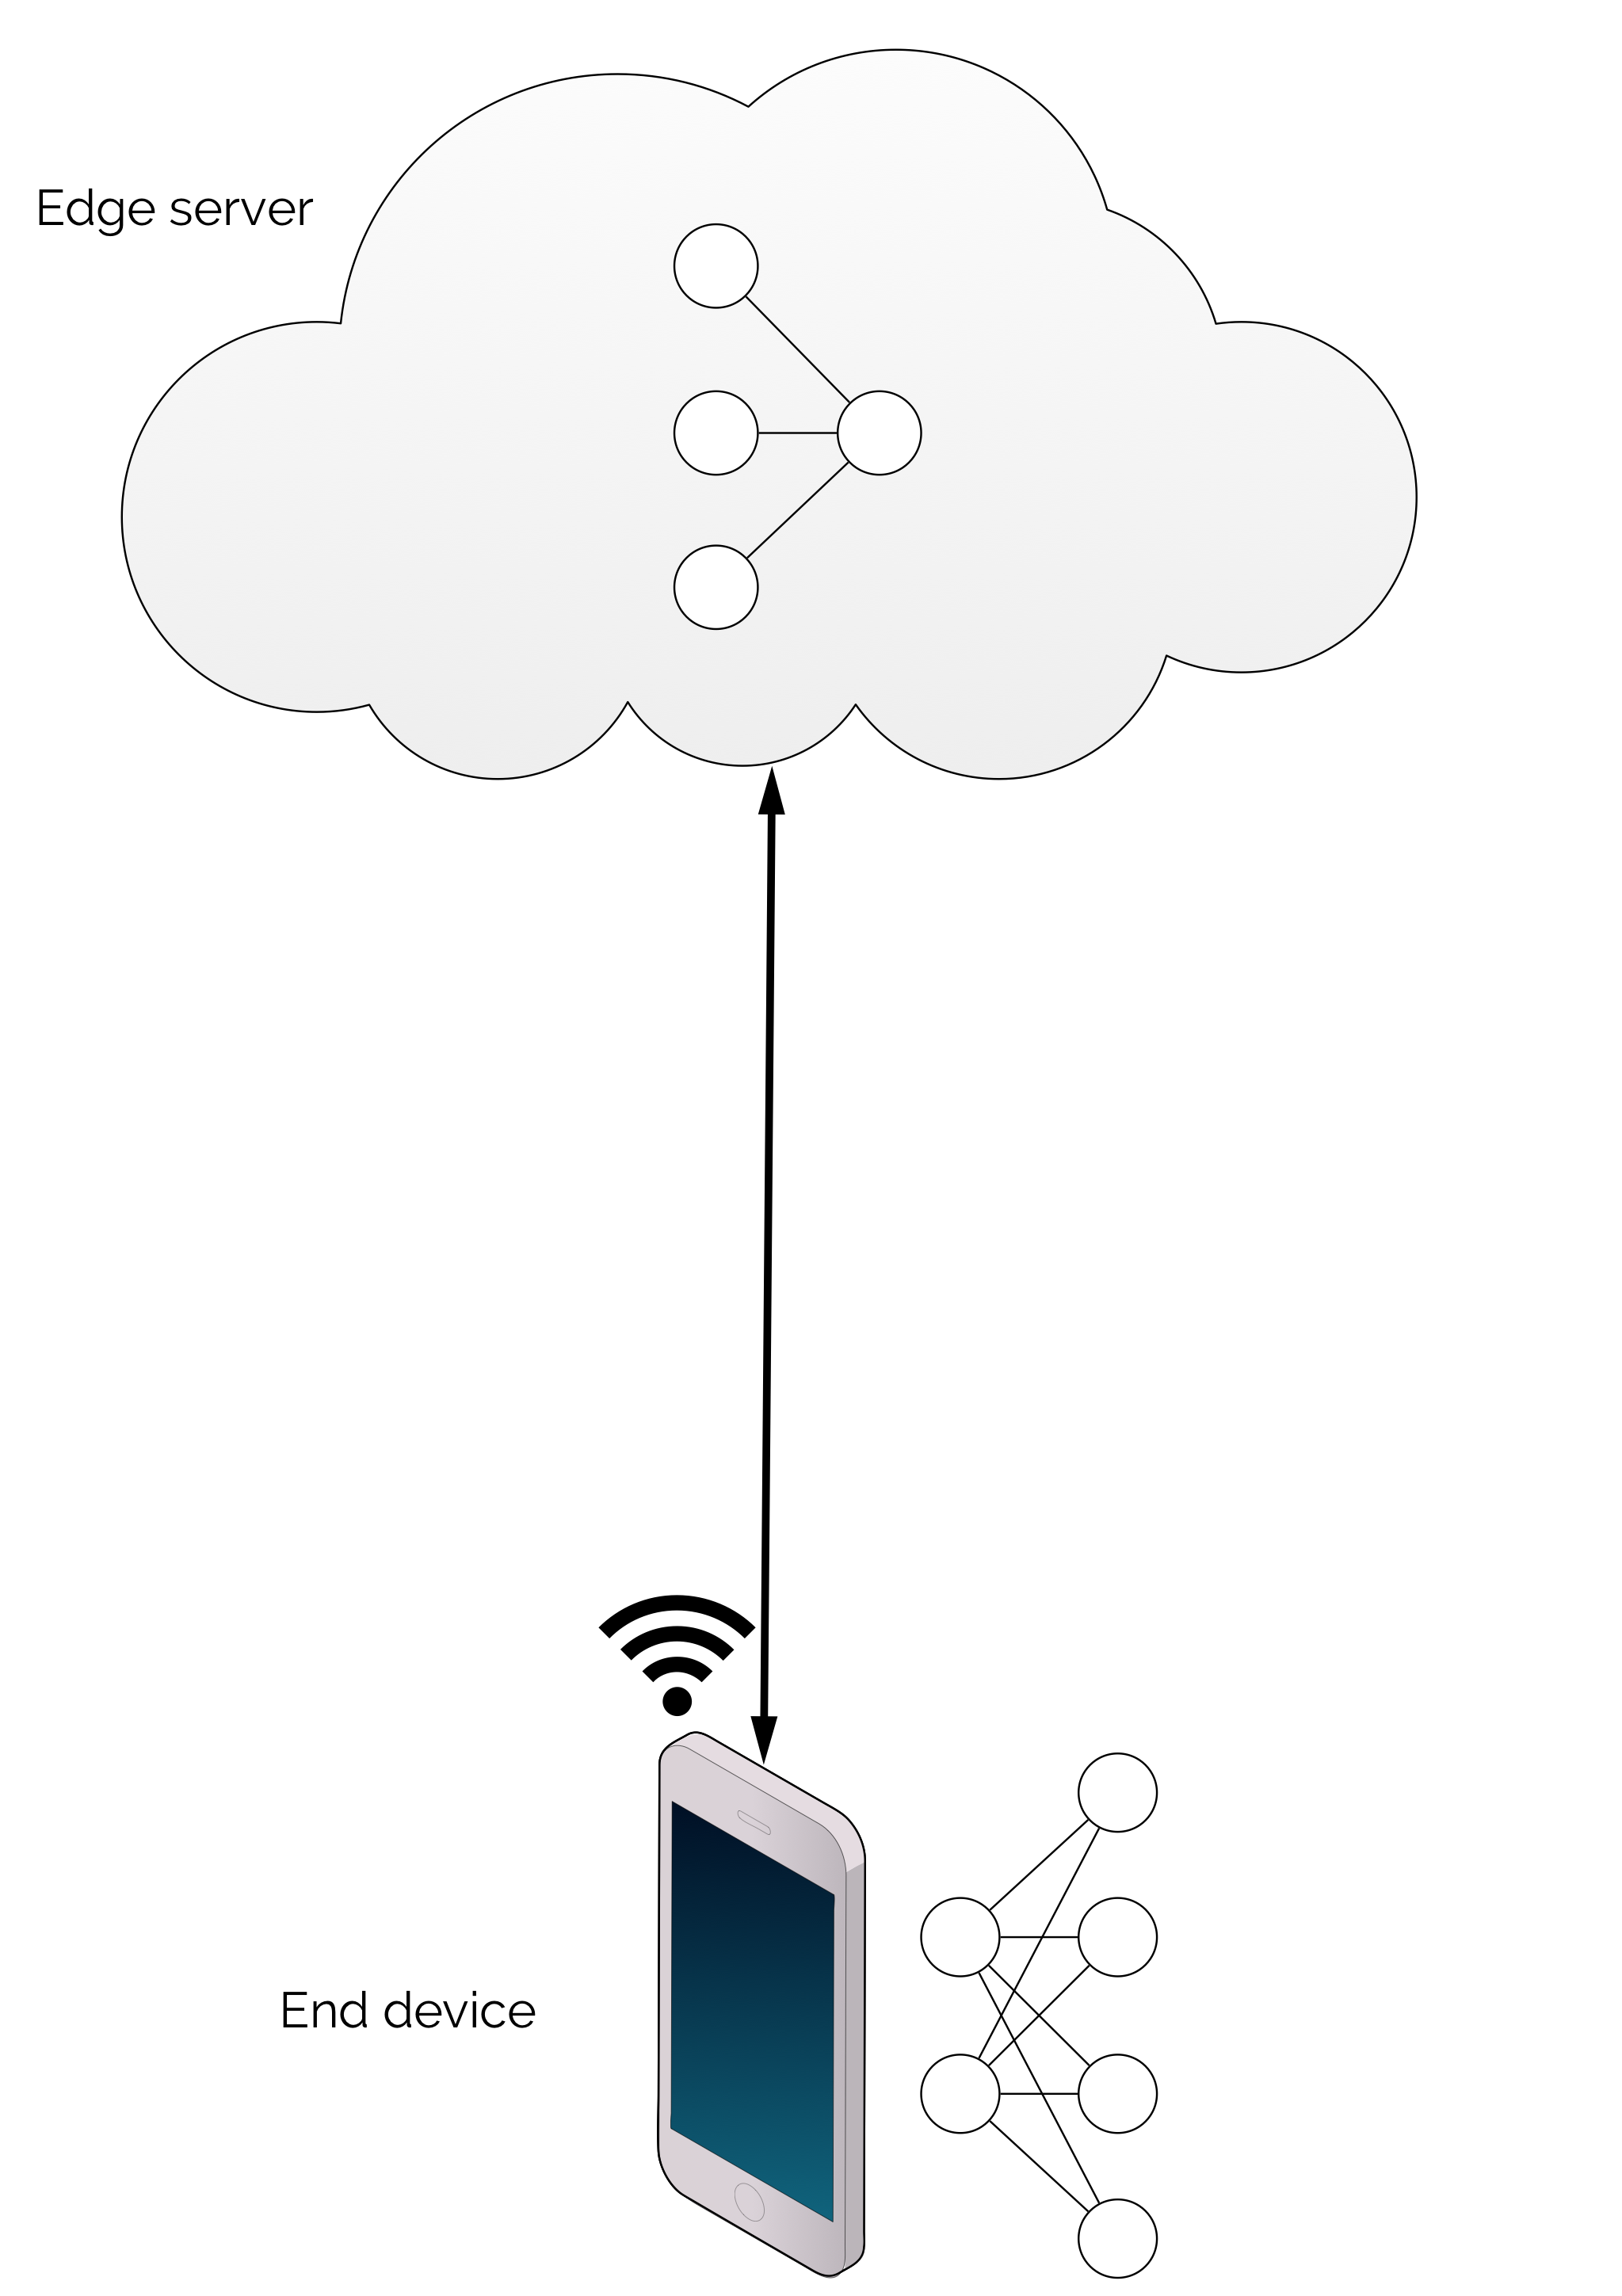
\includegraphics[width=\linewidth]{figures/models/edge_device}}
		\end{figure}
	\end{minipage}
	\begin{minipage}{0.5\linewidth}
		\centering
		\captionsetup[subfigure]{justification=centering}
		\begin{figure}
			\centering
			\subfloat[Collaborative Edge-Cloud\label{fig:edge-cloud-mode}]{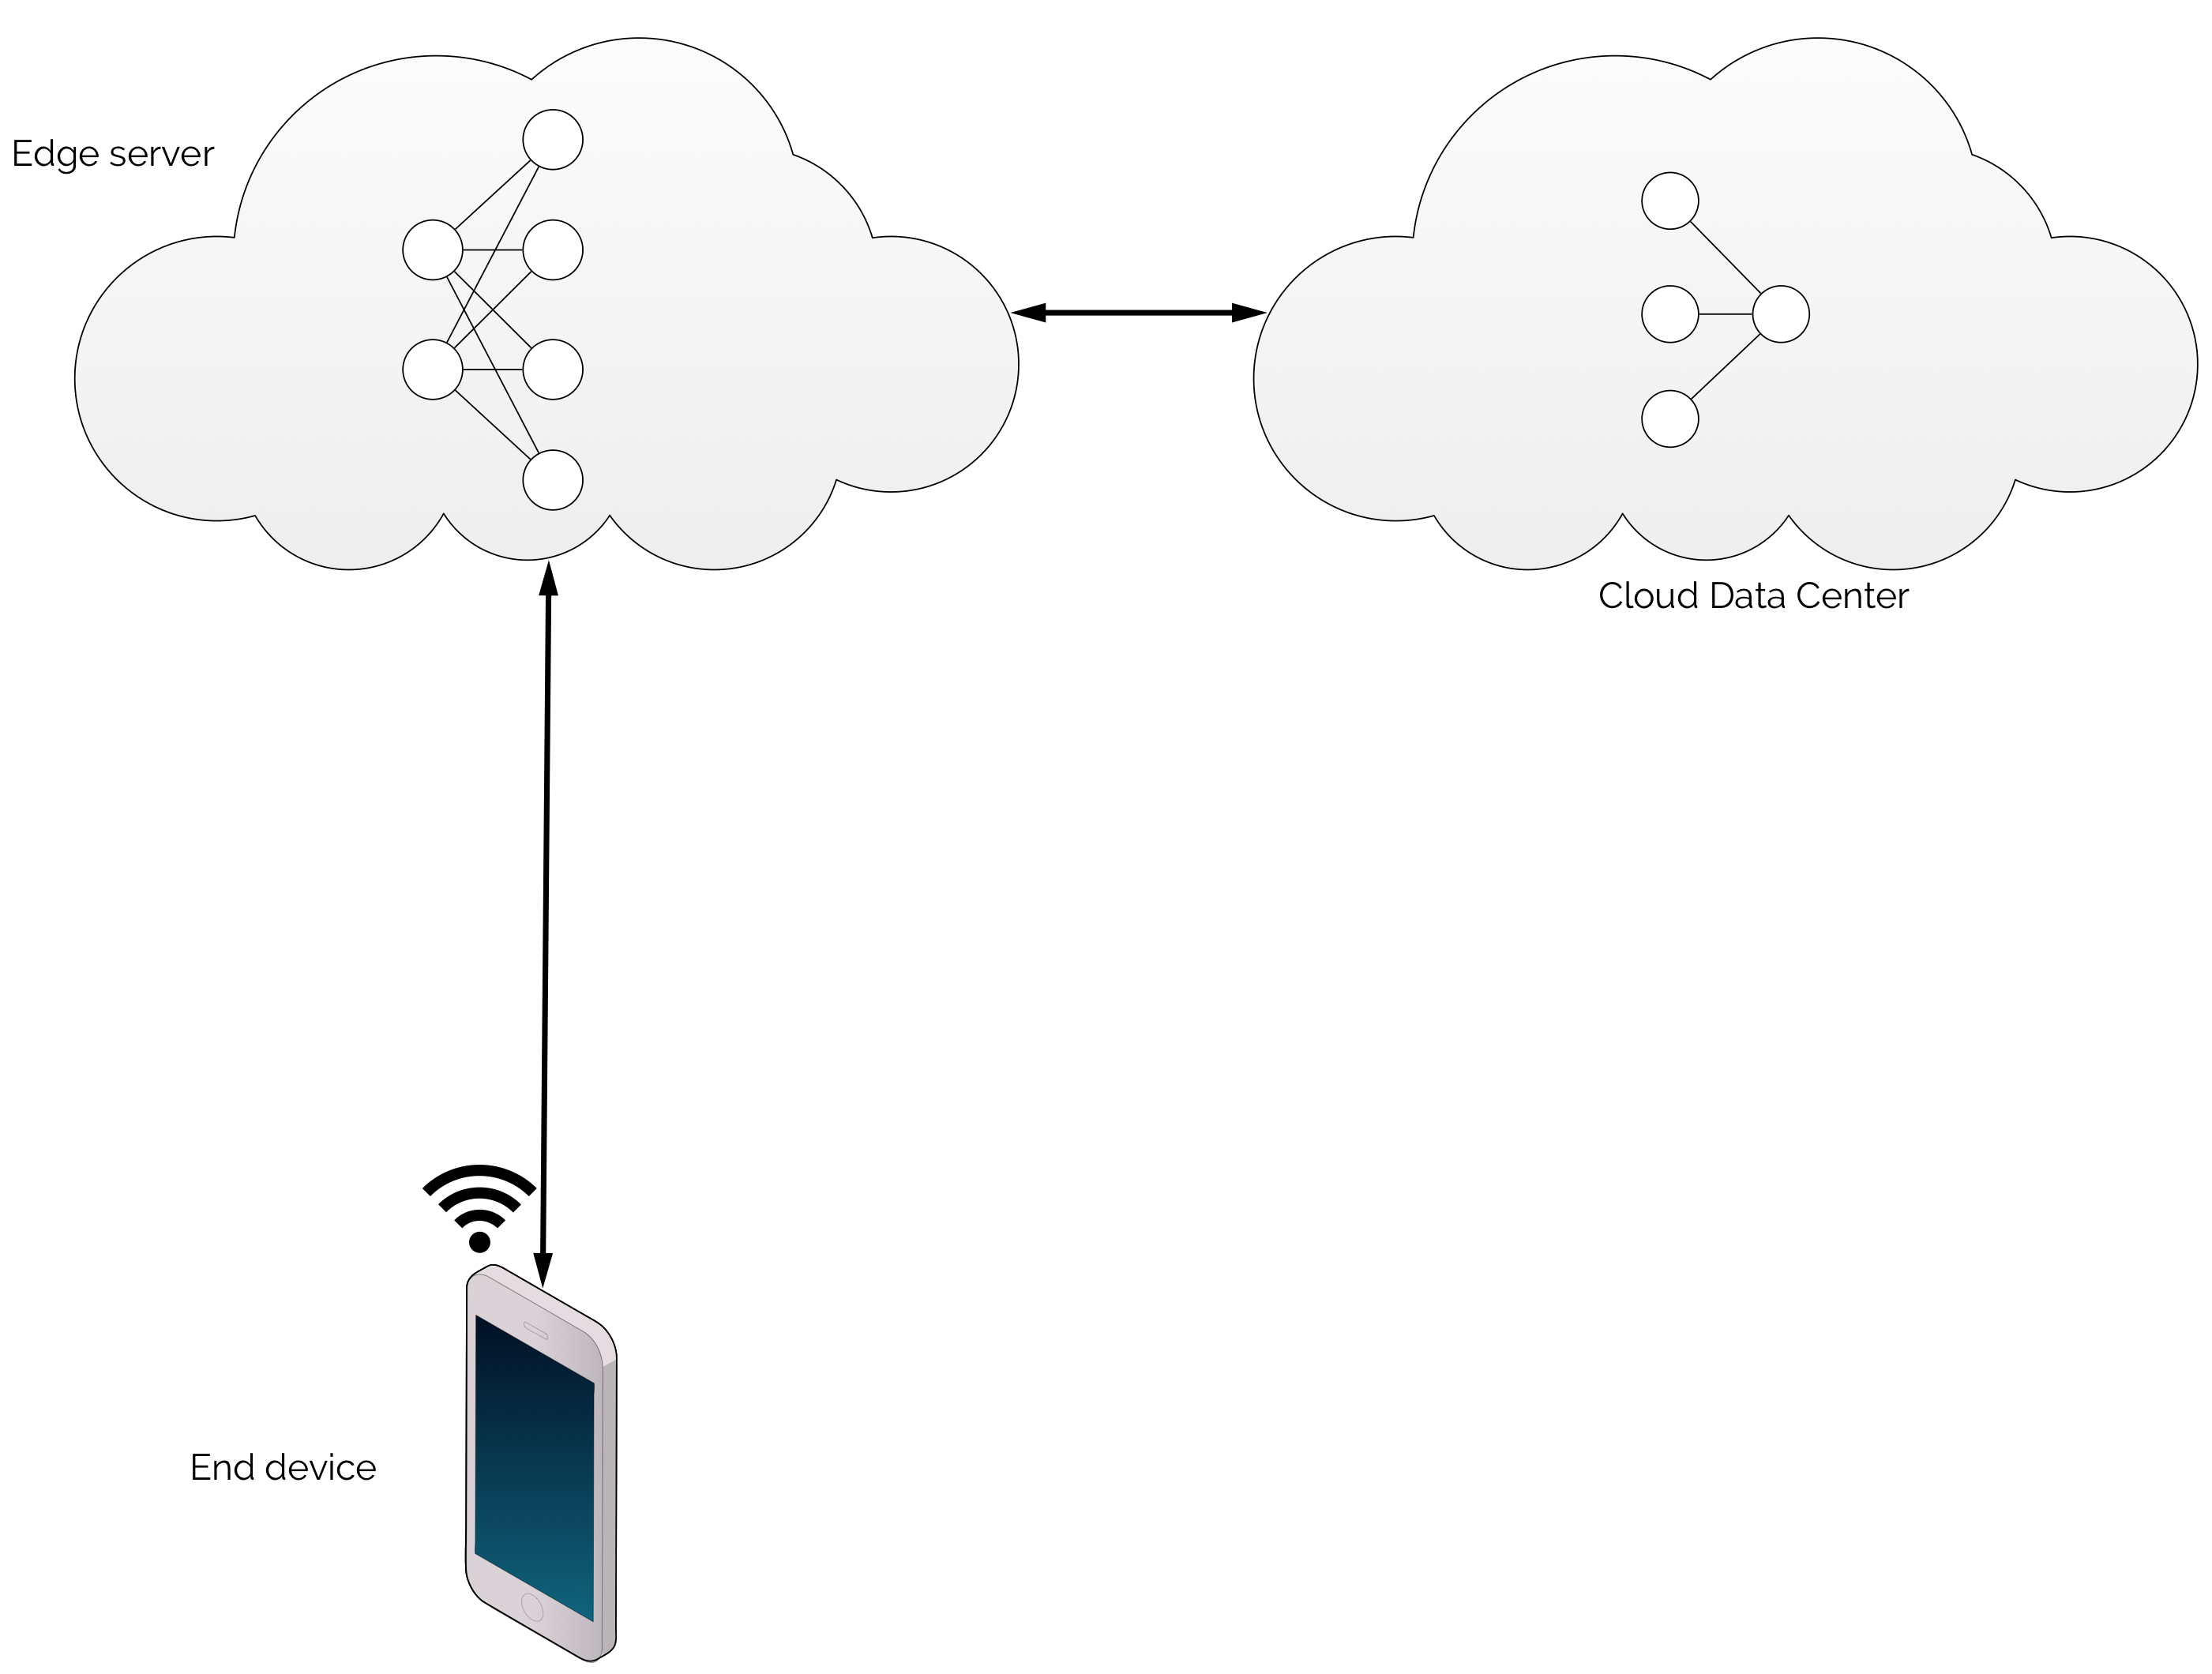
\includegraphics[width=\linewidth]{figures/models/edge_cloud}}
		\end{figure}
	\end{minipage}
	\hfill
	\begin{minipage}{0.45\linewidth}
		\textbf{\protect\subref{fig:edge-cloud-mode} \textsc{Collaborative Edge-Cloud}}
		\color{caption-color} \newline
		Resembles edge-device mode, however the model inference task is now partitioned between edge server and cloud data centers. The model is now reliant on edge server and data center computing resources, but even more so on network connection between edge and cloud. The scheme does too promote privacy, however only between edge and cloud and not in the local network at the edge. The two scheme could easily by combined to split inference between device, edge and cloud.
	\end{minipage}
	\caption[Edge-centric Architectures]{Edge-centric Architectures: \protect\subref{fig:device-based} device only execution, \protect\subref{fig:edge-based} edge only execution,\protect\subref{fig:edge-device-mode} edge and device partial execution, \protect\subref{fig:edge-cloud-mode} edge and cloud partial execution}
	\label{fig:edge_arch}
\end{figure}

The first two modes are the conventional schemes, which resembles the current \gls{di} and \gls{ci} frameworks, where all processing are done by one peer. The next two schemes presents collaborative architectures, where processing is divided for partial execution between the peers.
Moving model inference away from data centers with high-end specialized hardware offering tremendous amounts of computing power, to less powerful edge clusters or even just a standalone edge server, calls for improvements to model inference of extremely deep models, to adapt to the more diverse hardware landscape at the edge. In the next section, we present existing literature proposals of enabling technologies aiming at reducing the model inference time.

\section{Fast Inference} \label{sec:ei-fast-inference}

In this section enabling technologies for fast inference will be describes. Despite research in parallelism for \gls{cpu} and \gls{gpu}, efforts have been made in developing \gls{asic} or \gls{fpga}, i.e. specialized hardware such as Google's \gls{tpu} to further accelerete \gls{dnn}s, our main concern is model inference for real-time applications. We have chosen to present the technologies, that operate on a model level e.g., model architectures, -compression, -partitioning-, -selection, -early exit and layer skipping. We have chosen to omit technologies that operates on a infrastructural level e.g., edge caching, input filtering and support for multi-tenancy \cite{zhou_edge_2019}.

\small{
\begin{longtabu}{>{\bfseries}X|X[c]|X[c]|X[c]|X[c]|X[c]}
	\caption[]{} \label{tbl:fast-inference} \\
	\toprule
	\rowfont{\bfseries}
	Architecture & Category & Speed-Up method & Advantages & Disadvantages & Works \tabularnewline
	\hline
	\endfirsthead
	\multicolumn{3}{@{}l}{\textbf{\textcolor{black}{Table \ref{tbl:fast-inference}:}} continued}\\
	\toprule
	\rowfont{\bfseries}
	Architecture & Category & Speed-Up method & Advantages & Disadvantages & Works \tabularnewline
	\hline
	\endhead % all the lines above this will be repeated on every page
	\hline
	\multicolumn{3}{@{}l}{continued \ldots}\\
	\endfoot
	\hline
	\endlastfoot

	\multirow{5}{*}{Standalone} & Model Design & Innovative layer and operation design & Combineable, Memory footprint  & Accuracy cost & \cite{iandola_squeezenet:_2016,howard_mobilenets:_2017,sandler_mobilenetv2:_2018, zhang_shufflenet:_2017, ma_shufflenet_2018} \tabularnewline
	\tabucline{2-6}
	
	& Model Compression & Reduce model size & Adaptive, Combineable, Memory footprint & Accuracy cost &  \cite{hinton_distilling_2015,courbariaux_binaryconnect:_2015,courbariaux_binarized_2016,romero_fitnets:_2014} \tabularnewline	
	& & & & & \tabularnewline
	\tabucline{2-6}
	
	& Model Selection & Reduce depth overhead by selecting smaller model & Adaptive, Early exit & Accuracy cost, may require multiple \gls{dnn} inferences & \cite{bolukbasi_adaptive_2017, park_big/little_2015} \tabularnewline
	\tabucline{2-6}
	
	& Model Early Exit & Reduce depth overhead using less layers & Adaptive, Early exit, No additional inference, Multiple predictions & Accuracy cost, Possible lack of coarse level features & \cite{leroux_resource-constrained_2015,teerapittayanon_branchynet:_2016, berestizshevsky_sacrificing_2019, kaya_shallow-deep_nodate, huang_multi-scale_2017} \tabularnewline
	\tabucline{2-6}
	& Model Layer Skipping & Reduce depth overhead using less layers & Adaptive, Coarse level features & Accuracy cost, require additional reinforcement learning of skipping policies & \cite{wang_skipnet:_2017,wu_blockdrop:_2017} \tabularnewline
	\hline
	\multirow{3}{*}{Collaborative} & Model Partitioning & Reduce size of intermediate feature size to reduce communication latency & Utilize a more powerful device for heavy processing  & Accuracy cost, Compression aware training & \cite{kang_neurosurgeon:_2017,choi_near-lossless_2018, choi_deep_2018, eshratifar_bottlenet:_2019} \tabularnewline
	\tabucline{2-6}
	
	& Big/Little & Reduced depth and communication overhead of offlaoding using a small local model & Reduce unnecessary communication efforts & Accuracy cost, may require multiple \gls{dnn} inferences & \cite{park_big/little_2015} \tabularnewline \tabucline{2-6}
	
	& Distributed Exits & Reduced depth and communication overhead of offloading using local exits  &  Reduce unnecessary communication efforts, same inference task & Accuracy cost & \cite{leroux_cascading_2017,teerapittayanon_distributed_2017, li_edge_2018} \tabularnewline \tabucline{2-6}
	
	& & & & & \tabularnewline \tabucline{2-6}
	
	& & & & & \tabularnewline 

	\bottomrule
\end{longtabu}}

\subsection{Standalone Inference}

In this subsection efforts to reduce standalone inference time for \gls{dnn}s are explained. These effort are not particularly aimed at \gls{di}, \gls{ei} or \gls{ci}, but usable for either one standalone. 

\begin{enumdescript}
	\item[Model Design] To improve inference latency efforts have been made in designing \gls{dnn}s, that reduces the size of the model to more efficiently run on mobile and \gls{iot} devices. Most effort addresses  ways to reduce the number of parameters of the \gls{dnn}s, such as \gls{squeezenet} \cite{iandola_squeezenet:_2016}, that down samples the data size using convolutions to reduce the model size. Or by creating more efficient models, that reduces the amount of \gls{flop} required for the model. \gls{mobilenet}s \cite{howard_mobilenets:_2017,sandler_mobilenetv2:_2018} decomposes the convolution filters into simpler operations, thus reduces the amount of computations for the model- \gls{shufflenet}s \cite{zhang_shufflenet:_2017, ma_shufflenet_2018}, that uses a point-wise convolution operation and channel shuffling to reduce the amount of computations. Other efforts have been made to reduce the number of parameters for existing \gls{dnn} architectures using model compression.
	
	\item[Model compression]  is about finding a more compact or compressed way to represent the model. Pruning is probably the most widespread compression technique. Pruning can be used to create sparse networks, by removing the least contributing neurons and connections. Pruning have shown significant speed-ups with only a small loss in accuracy \cite{zhou_edge_2019}. The impact of compression is application dependent and can be applied to any pre-trained \gls{dnn} and in combination with other techniques \cite{cheng_survey_2017}.
	
	\begin{minipage}[t]{\linewidth}
		\centering
		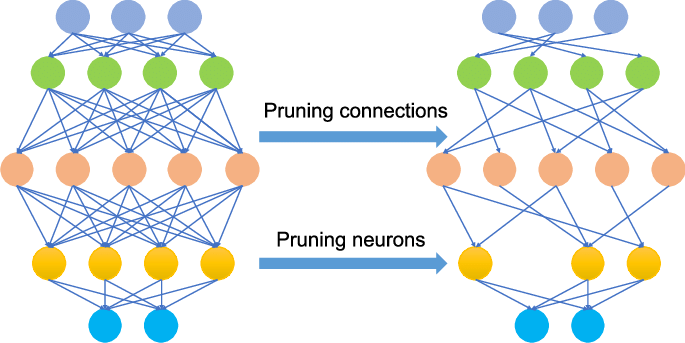
\includegraphics[width=.4\linewidth]{figures/articles/Pruning-a-neural-network}
		\captionof{figure}[\gls{dnn} Pruning]{Pruning conection and neurons source: \citetitle{chen_deep_2019} \cite{chen_deep_2019}}
	\end{minipage}
	
	Another compression technique is quantization. A more compact representation of a floating point is used to reduce the amount of bits needed for each weight of the model \cite{cheng_survey_2017}. The extreme case is binarization, where weights and activations are learned as a binary representations. In BinaryConnect \cite{courbariaux_binaryconnect:_2015} and \gls{bnn} \cite{courbariaux_binarized_2016} most arithmetic operations are replaced with bit-wise operations, thus greatly improving the power-efficiency and inference latency, however using binary weights in extremely deep network have also shown significant degradation of model accuracy \cite{cheng_survey_2017}.
	
	In \cite{hinton_distilling_2015} \gls{kd} has been proposed. \gls{kd} is a framework to train \gls{dnn} in a student-teacher paradigm. The student network are penalized using the output of an ensemble of teacher networks. \gls{kd} can be viewed as a compression of an ensemble of teacher network into a student network \cite{cheng_survey_2017}. 
	In \cite{romero_fitnets:_2014} \gls{fitnet} have been proposed as a method to train thinner and shallower student networks using a deeper teacher network. FitNet learns the student network to mimick the teacher network, however this approach require the softmax loss function, which limits its usage \cite{cheng_survey_2017}.  
	
	\item[Model Selection] Model selection is an approach to reduce inference by selecting an appropriately accurate model, hence not using an unnecessarily deep model, if a shallower model could give a satisfactory prediction. In \cite{bolukbasi_adaptive_2017} an adaptive model selection framework is proposed. The framework stacks three \gls{dnn} with increasing depth and increasingly higher accuracy models; \gls{alexnet}, \gls{googlenet} and \gls{resnet}50. 

	\begin{minipage}[t]{\linewidth}                              
		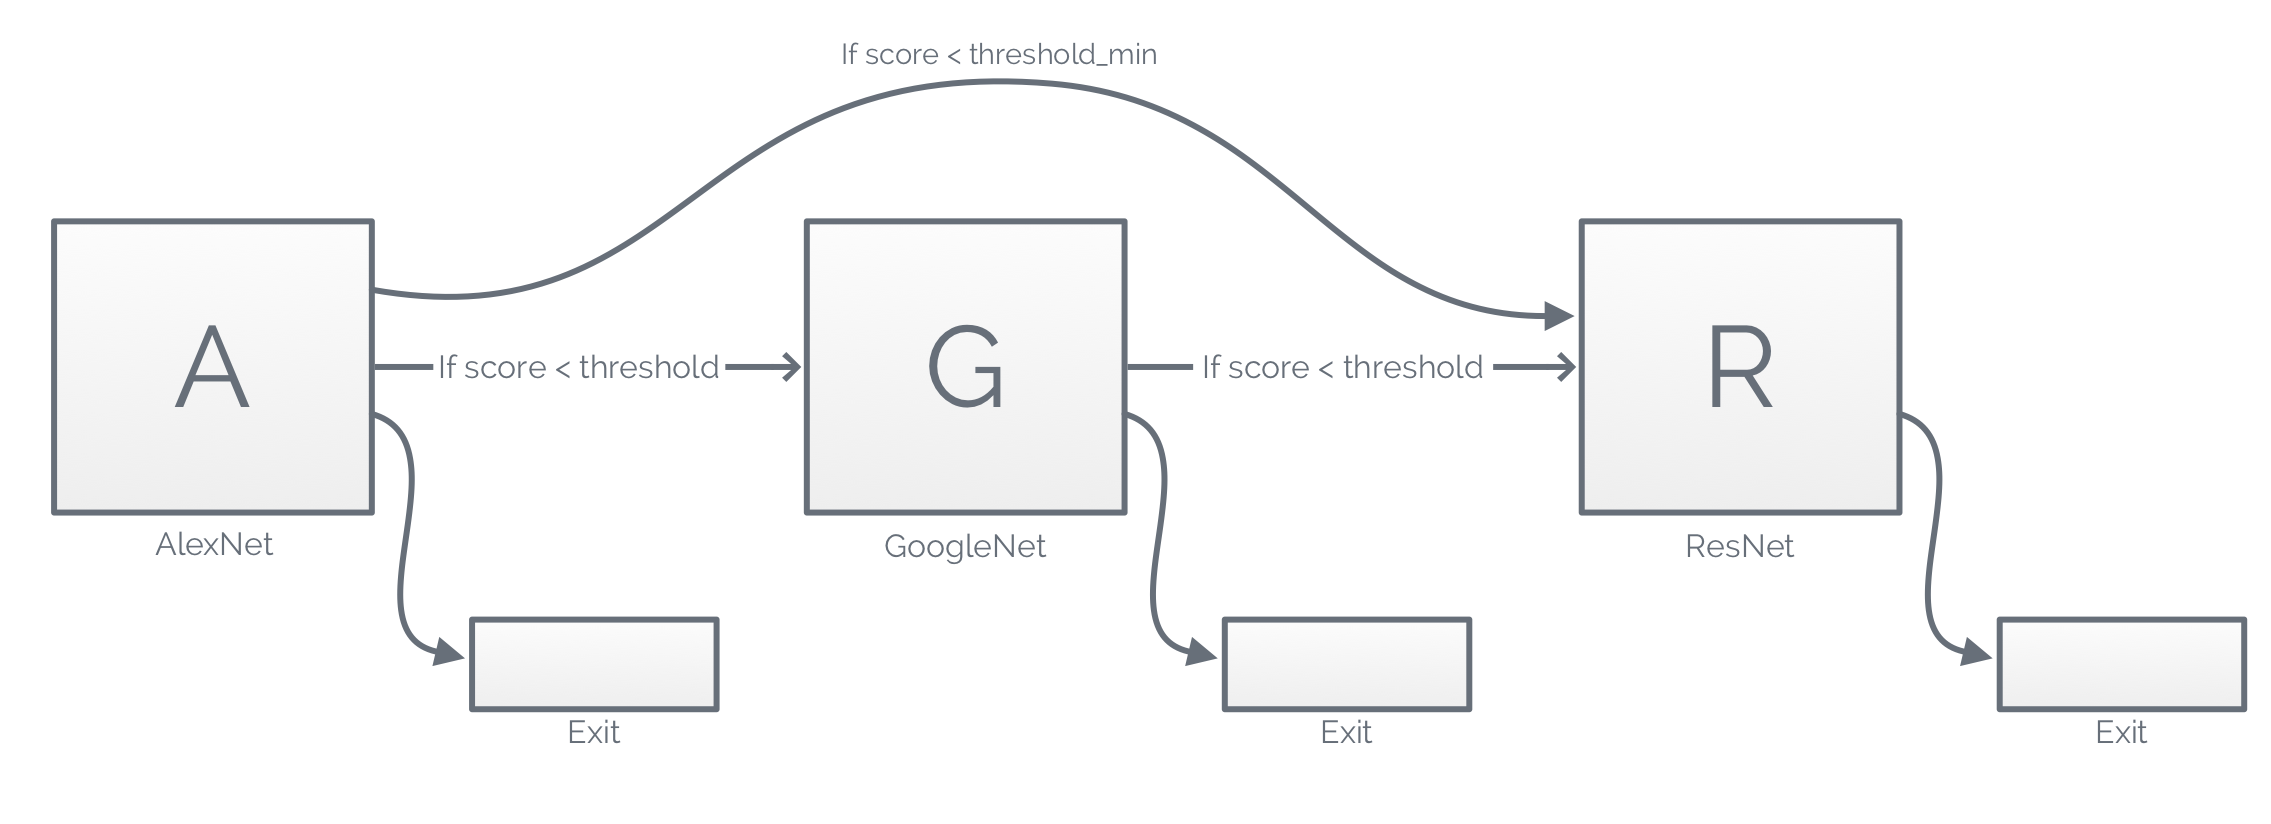
\includegraphics[width=\linewidth]{figures/models/adaptive}
		\captionof{figure}[Adaptive Neural Network]{Adaptive Neural Network using model selection}
	\end{minipage}
	
	The input is inferred to \gls{alexnet}, if the confidence scores is satisfactory the prediction is accepted, if not the framework decides to use either \gls{googlenet} or \gls{resnet}50 depending on a confidence threshold, however if the sample is inferred to \gls{googlenet} and the confidence is still unsatisfactory the sample is inferred to \gls{resnet}50 for final prediction. The work shows improvement of the average prediction time with only a small reduction in accuracy depending on the confidence threshold. However, for hard samples, since multiple model are introduced, the inference time is increased, as well as the computational cost and memory consumption, thus such model selection approach seems overwhelming to introduce on a constraint end device. Yet it may be feasible to offload to the edge using a Big/Little setup.
	
	To obtain faster inference Big/Little \gls{dnn} \cite{park_big/little_2015} implements a hybrid edge architecture of device-only and selective offloading for edge-only processing. It runs a shallower, albeit less accurate model on device, and a deep and more accurate model on the edge server, as illustrated by figure \ref{fig:big/little-dnn}. 
	
	\begin{minipage}[t]{\linewidth}                              
		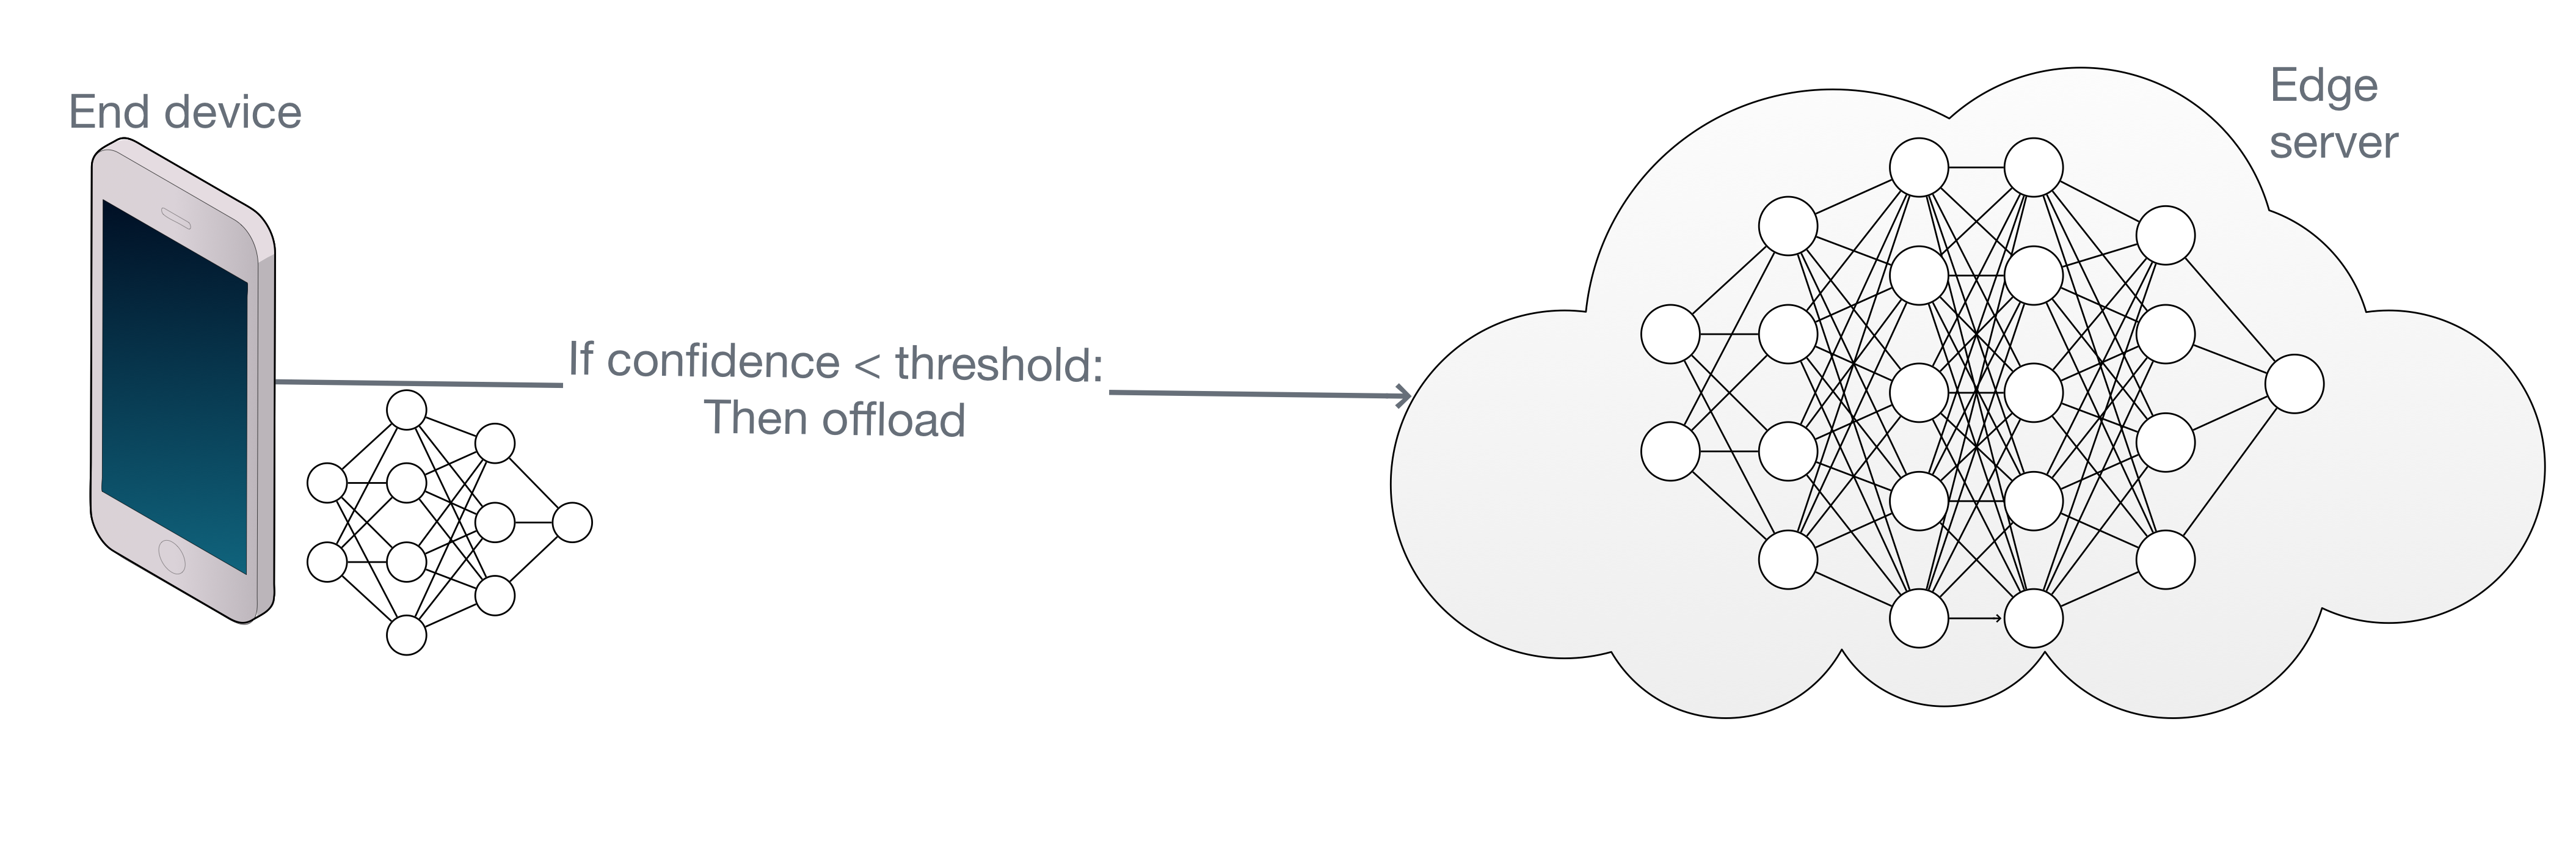
\includegraphics[width=\linewidth]{figures/models/big_little_dnn}
		\captionof{figure}[Big/Little \gls{dnn} architecture]{Big/Little \gls{dnn}, a hybrid edge architecture. An on-device model is used to selectively offload to a more complex model hosted on an edge server.}
		\label{fig:big/little-dnn}
	\end{minipage}
	
	If the prediction confidence of the little model is unsatisfactory, a decision is made to offload to the big model on the edge server. If a lot of samples are able to be correctly classified locally, a speed-up is gained. However, the down-side of this approach is, if too many samples require the big model to satisfy a certain confidence threshold, a lot of work is wasted on the on-device prediction. Although Big/Little \gls{dnn} obtain good results on energy savings and inference latency, other approaches such as early exiting, tries to reduce wasted computation of the little \gls{dnn}, by creating multiple exits in an existing model.
	
	\item[Model Early Exit] Cascading \gls{dnn} \cite{leroux_resource-constrained_2015} and \gls{branchynet} \cite{teerapittayanon_branchynet:_2016} are both early exiting frameworks for fast inference using \gls{dnn}s. Research have shown, that only a few number of samples actually require extremely deep models to be correctly classified. The frameworks, illustrated in figure \ref{fig:branchynet}, adds a cascade of intermediate classifiers, or branch exits to the \gls{dnn}, that allow samples with a confidence higher than a selected threshold to be classified and exit the inference process prematurely. Other samples may require a later exit to obtain a high enough confidence score, or perhaps the entire depth of the model. The selection of an early exit threshold resembles model selection, if a too high threshold is selected, only a few sample might be able to exit the model at an early exit. If too low a threshold a lot of samples will exit the model and be incorrectly classified, thus degrading the model accuracy. 

	\begin{minipage}[t]{\linewidth}    
		\centering                          
		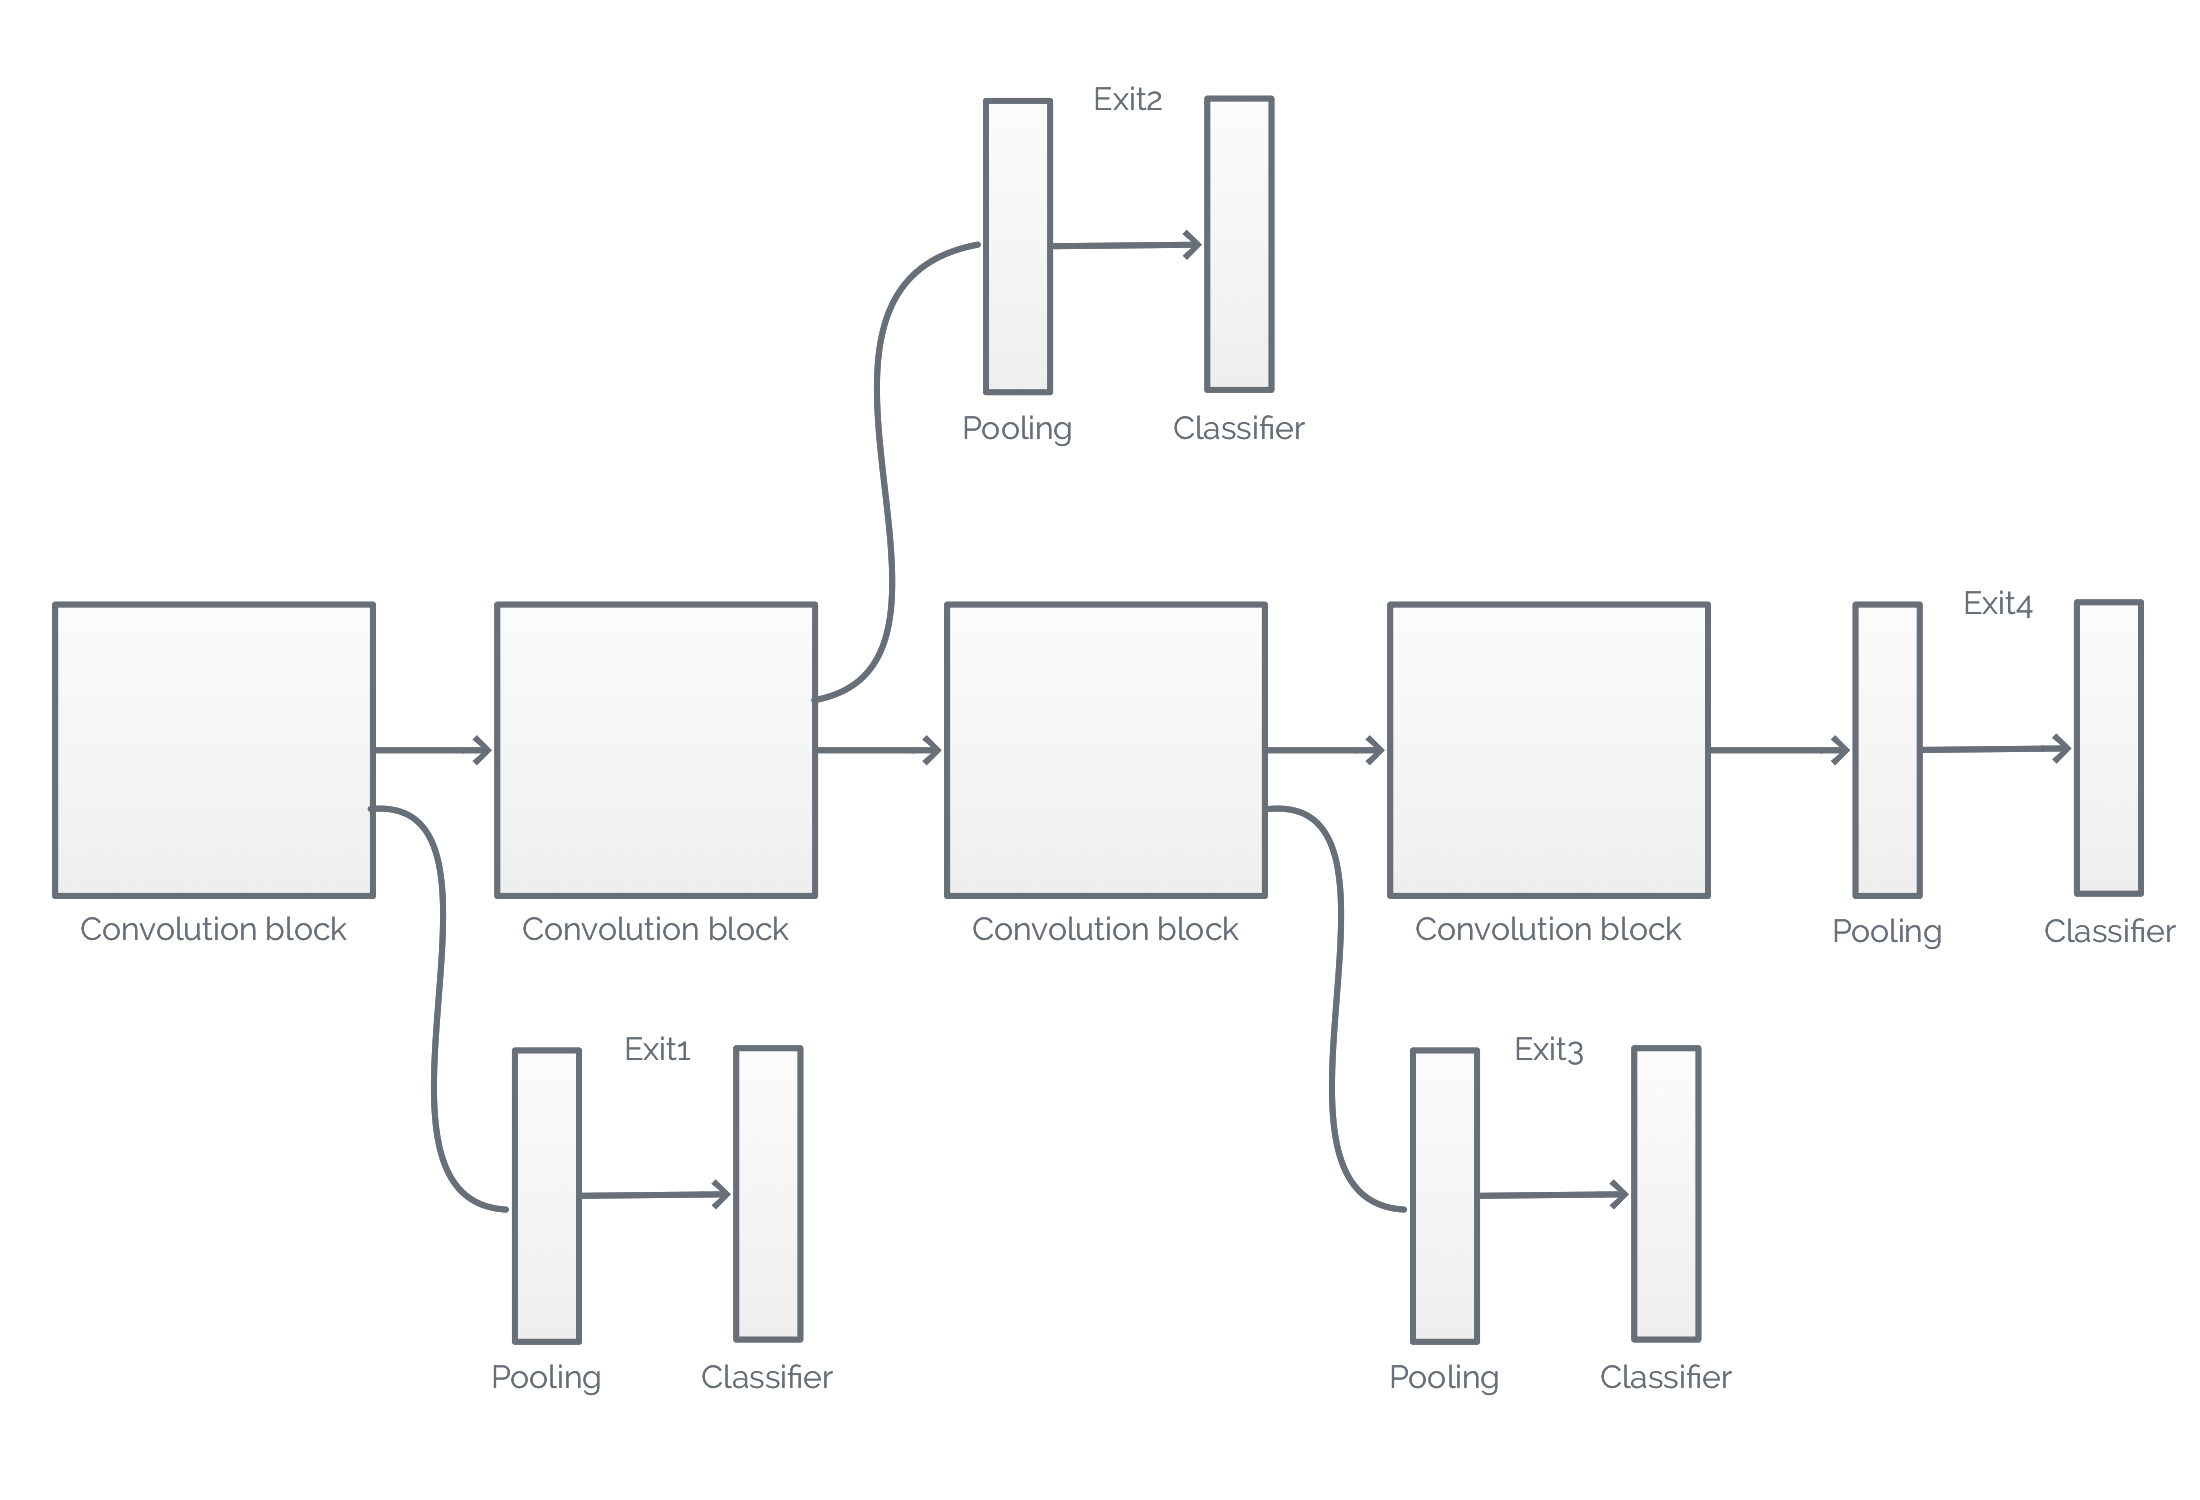
\includegraphics[width=.8\linewidth]{figures/models/branchy}
		\captionof{figure}[BranchyNet Architecture]{BranchyNet Architecture}
		\label{fig:branchynet}
	\end{minipage}

	Our work is based on standalone early exit \gls{dnn}s. Early exit is elaborated upon in section \ref{sec:ee-theory}.
	
	\item[Model Layer Skipping] Other approaches to reduce inference time of \gls{dnn} involve mechanism for skipping certain layers. SkipNet \cite{wang_skipnet:_2017} is a framework for adding dynamic decision for skipping layers. 
	
	\begin{minipage}[t]{\linewidth}    
		\centering                          
		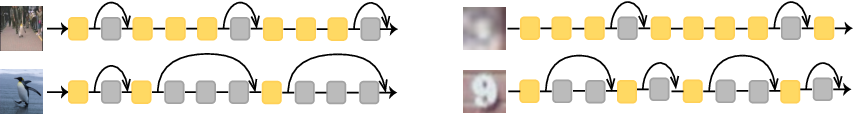
\includegraphics[width=.8\linewidth]{figures/models/skipnet}
		\captionof{figure}[SkipNet]{SkipNet}
	\end{minipage}
	
	The framework adds complexity to the model by introducing skipping gates between intermediate layers of the network. SkipNet is trained using a hybrid of supervised learning and reinforcement learning. The classification is learnt as a usual supervised problem using labeled data. The skipping policies are learnt using reinforcement learning by rewarding skipping decisions, that have little impact on classification accuracy. The work shows, that only a small fraction of inputs actually require these extremely deep models, thus SkipNet is able to reduce the computational cost by 30\% of \gls{resnet}101 on \gls{ilsvrc2012}. 
	
	BlockDrop \cite{wu_blockdrop:_2017} is another approach to learn skipping policies. However, instead of adding intermediate skipping gates for dynamic local decisions, BlockDrop trains a global policy network, that selectively chooses which model depth to use. BlockDrop is in fact a learned model selection framework, where the selection of models is not based on a confidence output of a smaller model, but on a \gls{dnn} trained to predict the complexity of an input sample. 
	
	
	\begin{minipage}[t]{\linewidth}    
		\centering
		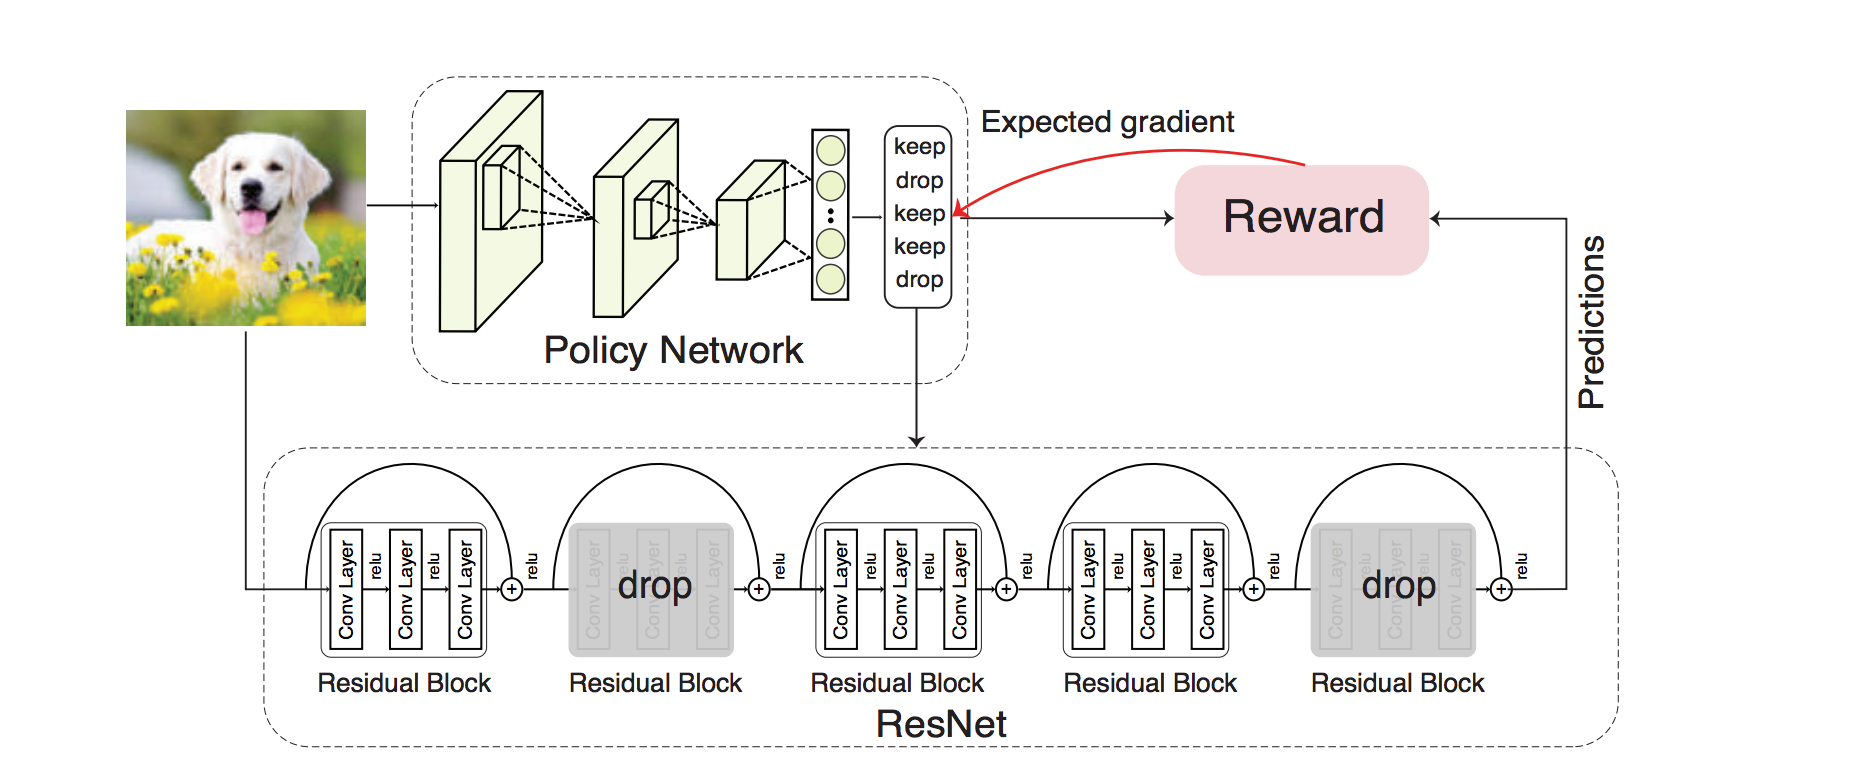
\includegraphics[width=\linewidth]{figures/models/blockdrop}
		\captionof{figure}[BlockDrop]{BlockDrop}
	\end{minipage}
	
	The policy network is similarly trained using reinforcement learning. The training shows, which classes are easy and which are hard. SkipNet and BlockDrop could both be used in an edge-device mode such as a Big/Little \cite{park_big/little_2015} setup. Particularly BlockDrop where the inexpensive policy network is run by an end device to selective choose among a smaller model on-device or a larger model on an edge server to avoid wasteful executions.
	
	We study early exiting model in this thesis, due to its flexible nature to prematurely exit samples useful for time-critical application with stringent deadlines. In the next chapter early exiting is elaborated upon and used for experiments.
	


\end{enumdescript}

\subsection{Collaborative Inference}

In this subsection we present efforts at reducing inference time for collaborative architectures. Instead of solely executing a \gls{dnn} in the cloud, edge or on device, the computing resources collaborates to boost inference time. Collaborative inference of a conventional \gls{dnn} is also known as model partitioning.

%Since early exiting less computation is wasted, if offloading is necessary after an exit compared to a Big/Little model selection setup. As less computation is needed and a smaller representation of input data can be obtained, thus less data must be offloaded to the edge server.
\begin{enumdescript}
	\item[Model partitioning] 
	Splitting a model is an inherent nature of sequential \gls{dnn}s. The inference process can be stopped at any layer. The intermediate output after the last executed layer are transferred over the network, and the inference continues at the next layer on an edge server, as shown in figure \ref{fig:offlaoding}.
	
	\begin{minipage}[t]{\linewidth}    
		\centering
		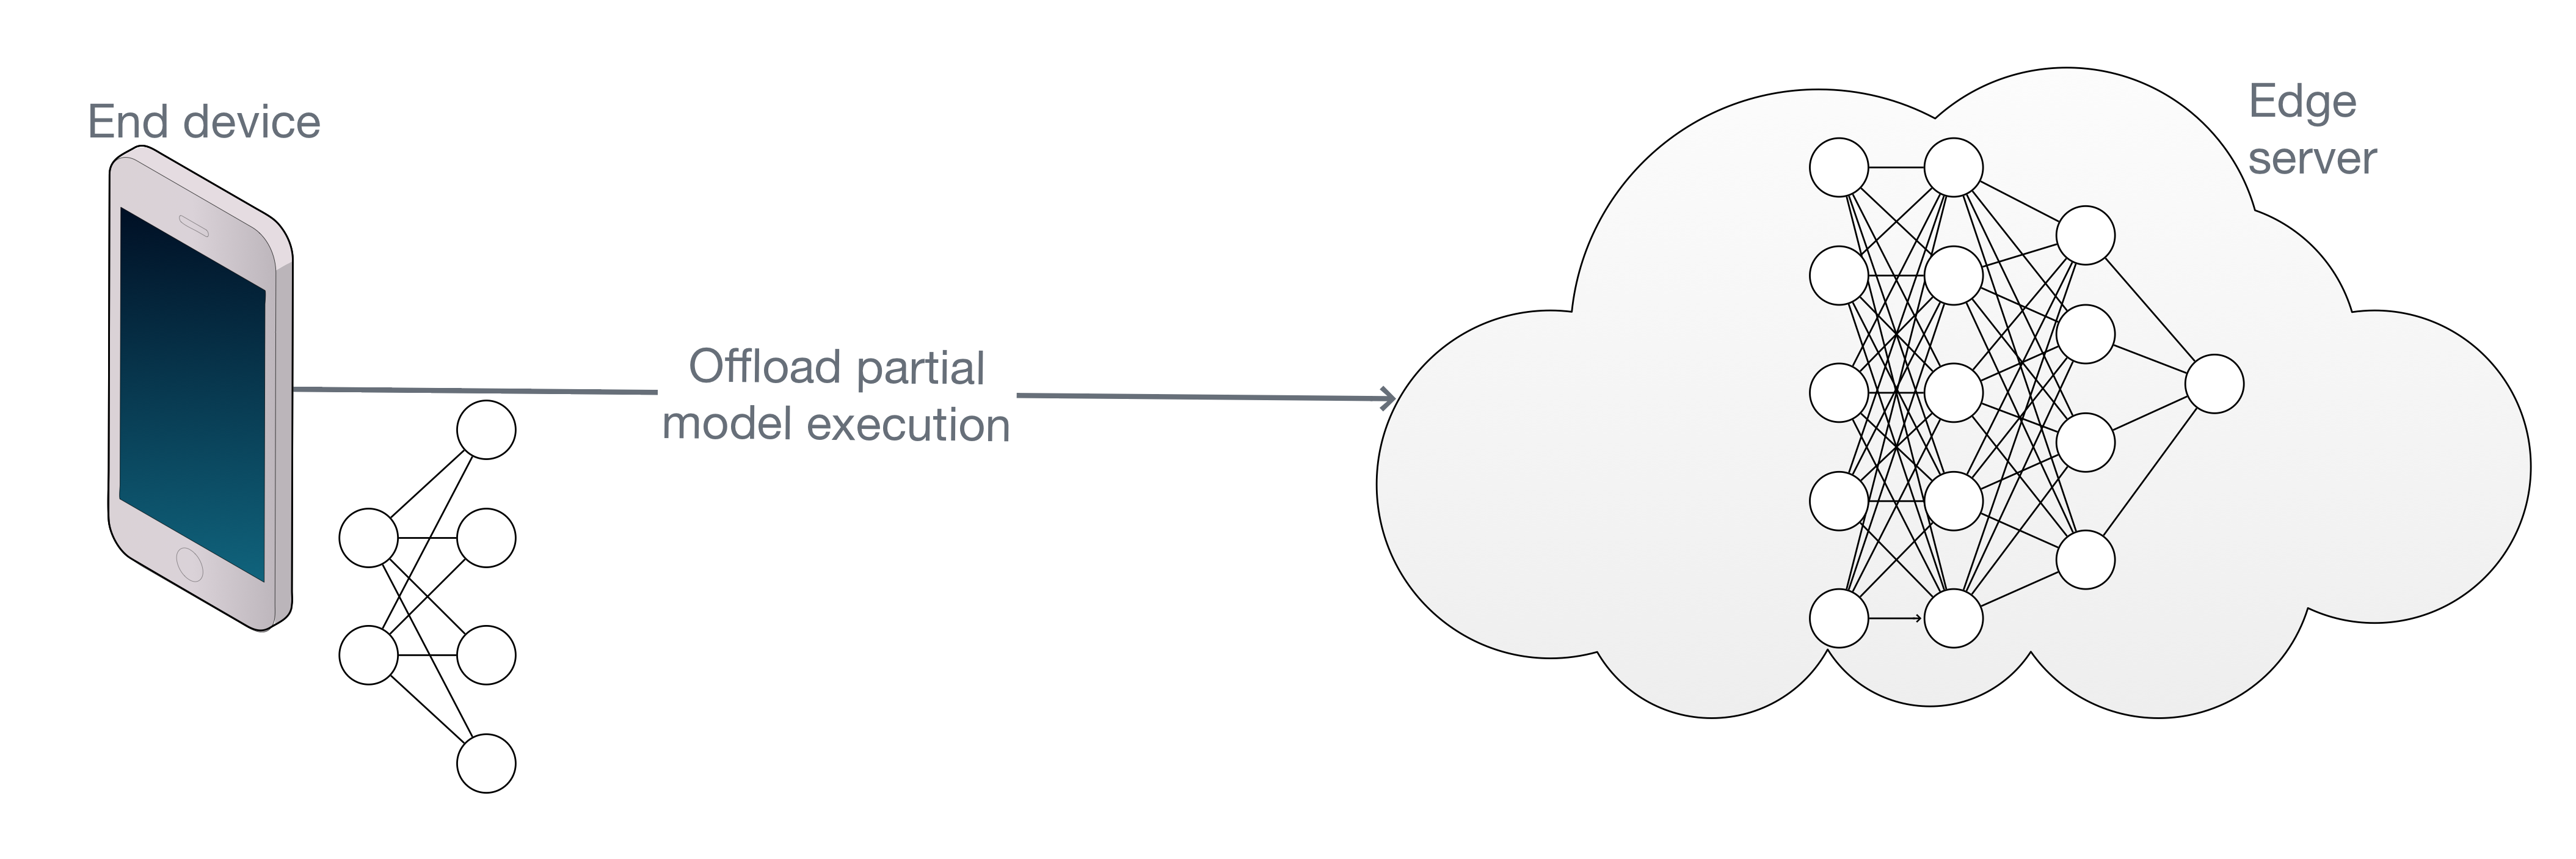
\includegraphics[width=\linewidth]{figures/models/partitioning}
		\captionof{figure}[Model partitioning]{Edge-Device model partitioning run part of the model on-device and offload the rest to edge processing. Network partitioning utilize the assumption, that at some later point in the \gls{dnn} a smaller representation of the data is found, illustrated by the gradually decreasing model layers, to reduce the communication bottleneck. }
		\label{fig:offlaoding}
	\end{minipage}
	
	Neurosurgeon \cite{kang_neurosurgeon:_2017} is a lightweight partitioning scheduler, that uses knowledge of the individual layers of the \gls{dnn} to effectively reduce inference latency. Communication delay is the bottleneck in such an offloading application, hence a smaller representation of the input data is needed, however the layers producing a smaller output than the original input, typically lies deep within the network. Neurosurgeon construct regression models for per layer execution time and output data size of the \gls{dnn}. The regression model are used to decide the best partition of the \gls{dnn} based on available communication data rate. The work is based on cloud intelligence setup and shows, that the conventional cloud-only approach is actually insufficient due to different low data rate connections to cloud data center and the trend that more mobile device is being equipped with \gls{gpu}s. 
	% Evidently moving computation to the edge reduces the communication latency. 
	
	Efforts have been made to reduce communication overhead, when splitting \gls{dnn}s to run in a collaborative scheme. One of which is compression of intermediate features before offloading to cloud or edge \cite{choi_deep_2018}. The paper shows, that lossless compression has, as expected, no impact on accuracy. However, bit saving is also rather limited. Lossy compression, on the other hand, results in 70\% bit savings, but also have negative impact of model accuracy. To compensate a compression aware training have been proposed. The follow up paper \cite{choi_near-lossless_2018} propose a novel compression technique, especially designed for deep features i.e. the output of an intermediate \gls{dnn} layers, and with significantly higher bit savings compared to conventional image compression algorithms such as JPEG. Alternatively, methods such as \gls{bottlenet} proposes novel \gls{dnn} module, that creates a low dimensional representation of the output features, able to be restored to original dimensionality. 
	
	
	\begin{minipage}[t]{\linewidth}    
		\centering
		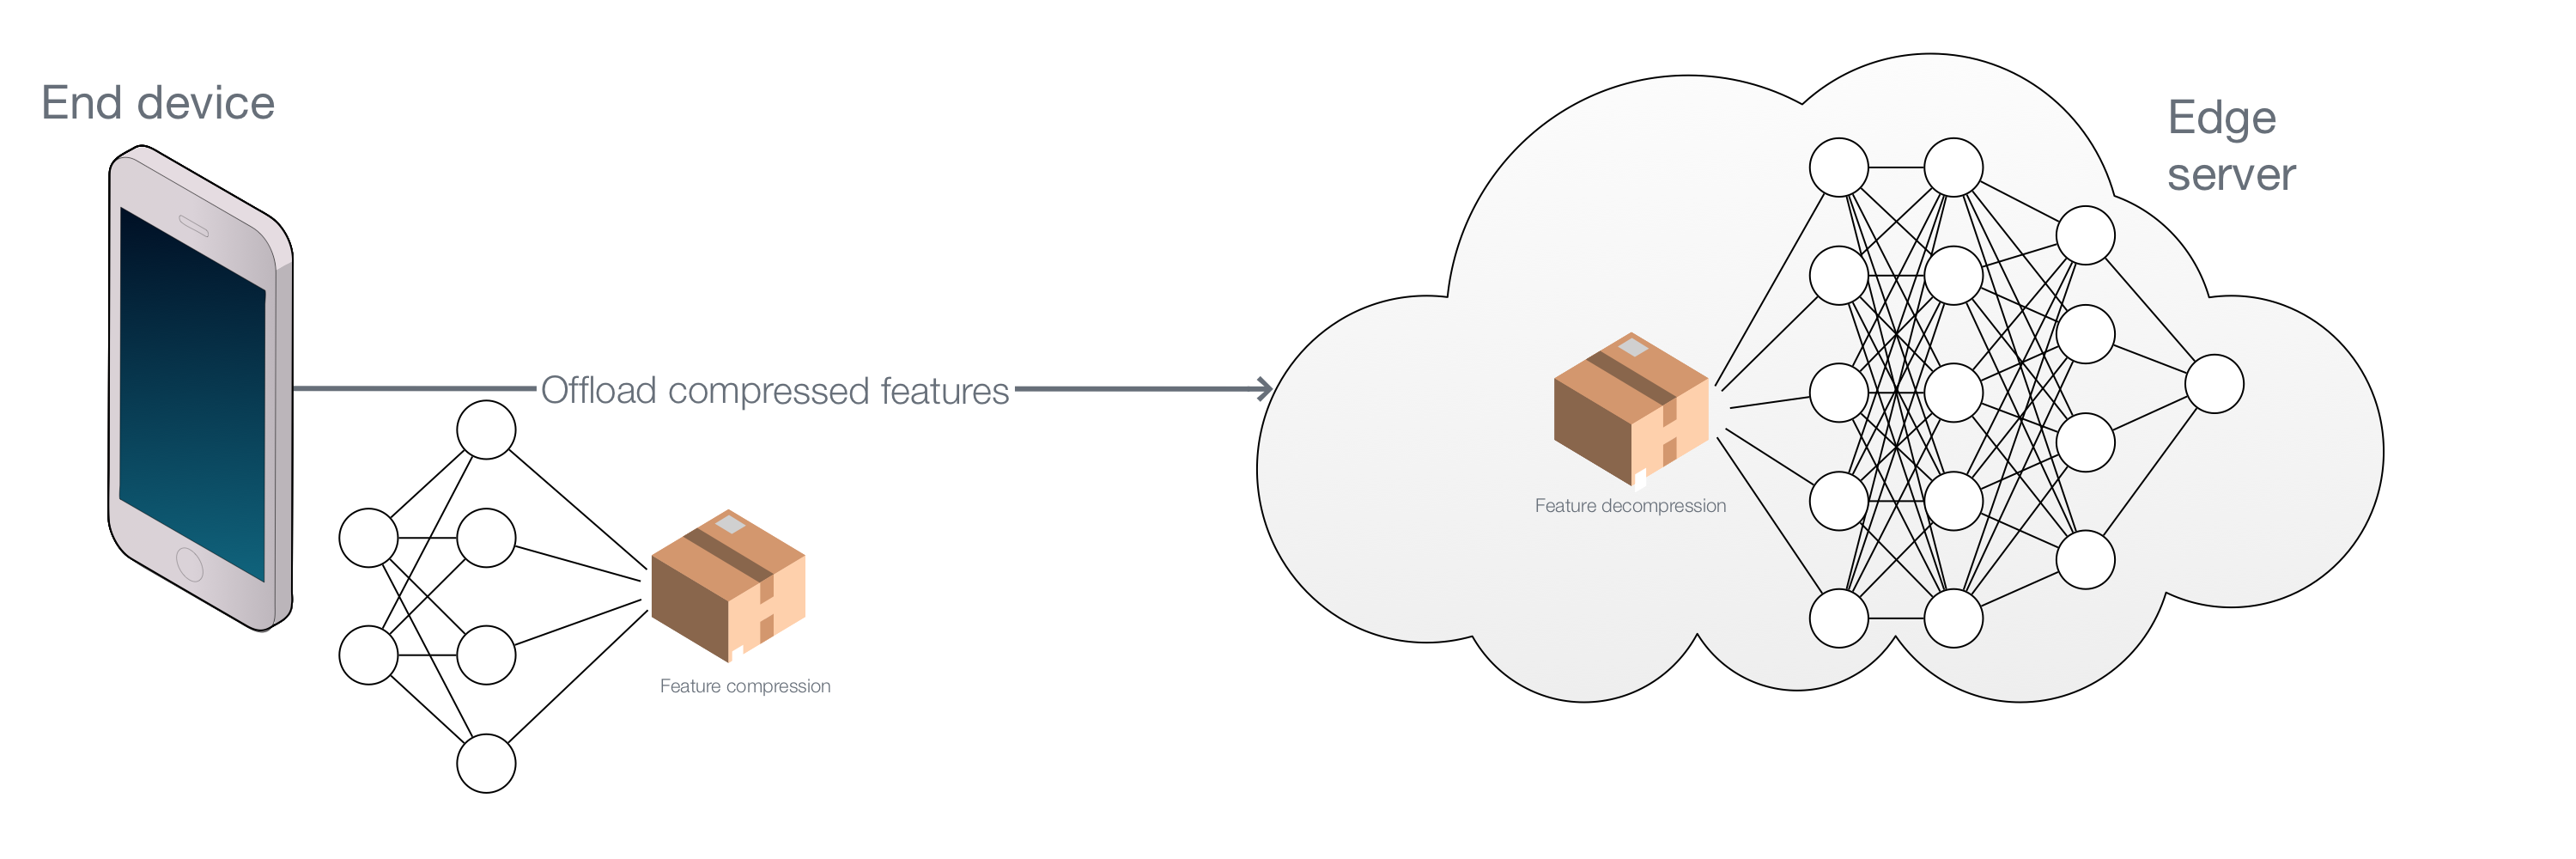
\includegraphics[width=\linewidth]{figures/models/compressed}
		\captionof{figure}[Feature compression]{Feature compression}
	\end{minipage}
	
	\gls{bottlenet} \cite{eshratifar_bottlenet:_2019} is a novel neural network module. Client-side it consists of a reduction unit and a compressor unit and server-side of a decompressor unit and restoration unit. The reduction unit creates a smaller representation of intermediate features by applying spatial- and channel-wise convolution. The compressor uses lossy JPEG compression and sends the data to the server. The server decompresses the received data and the restoration unit restores the intermediate feature using channel- and spatial-wise deconvolution, to get the required input size for the next layer in the \gls{dnn}.
	
	\begin{minipage}[t]{\linewidth}
		\centering
		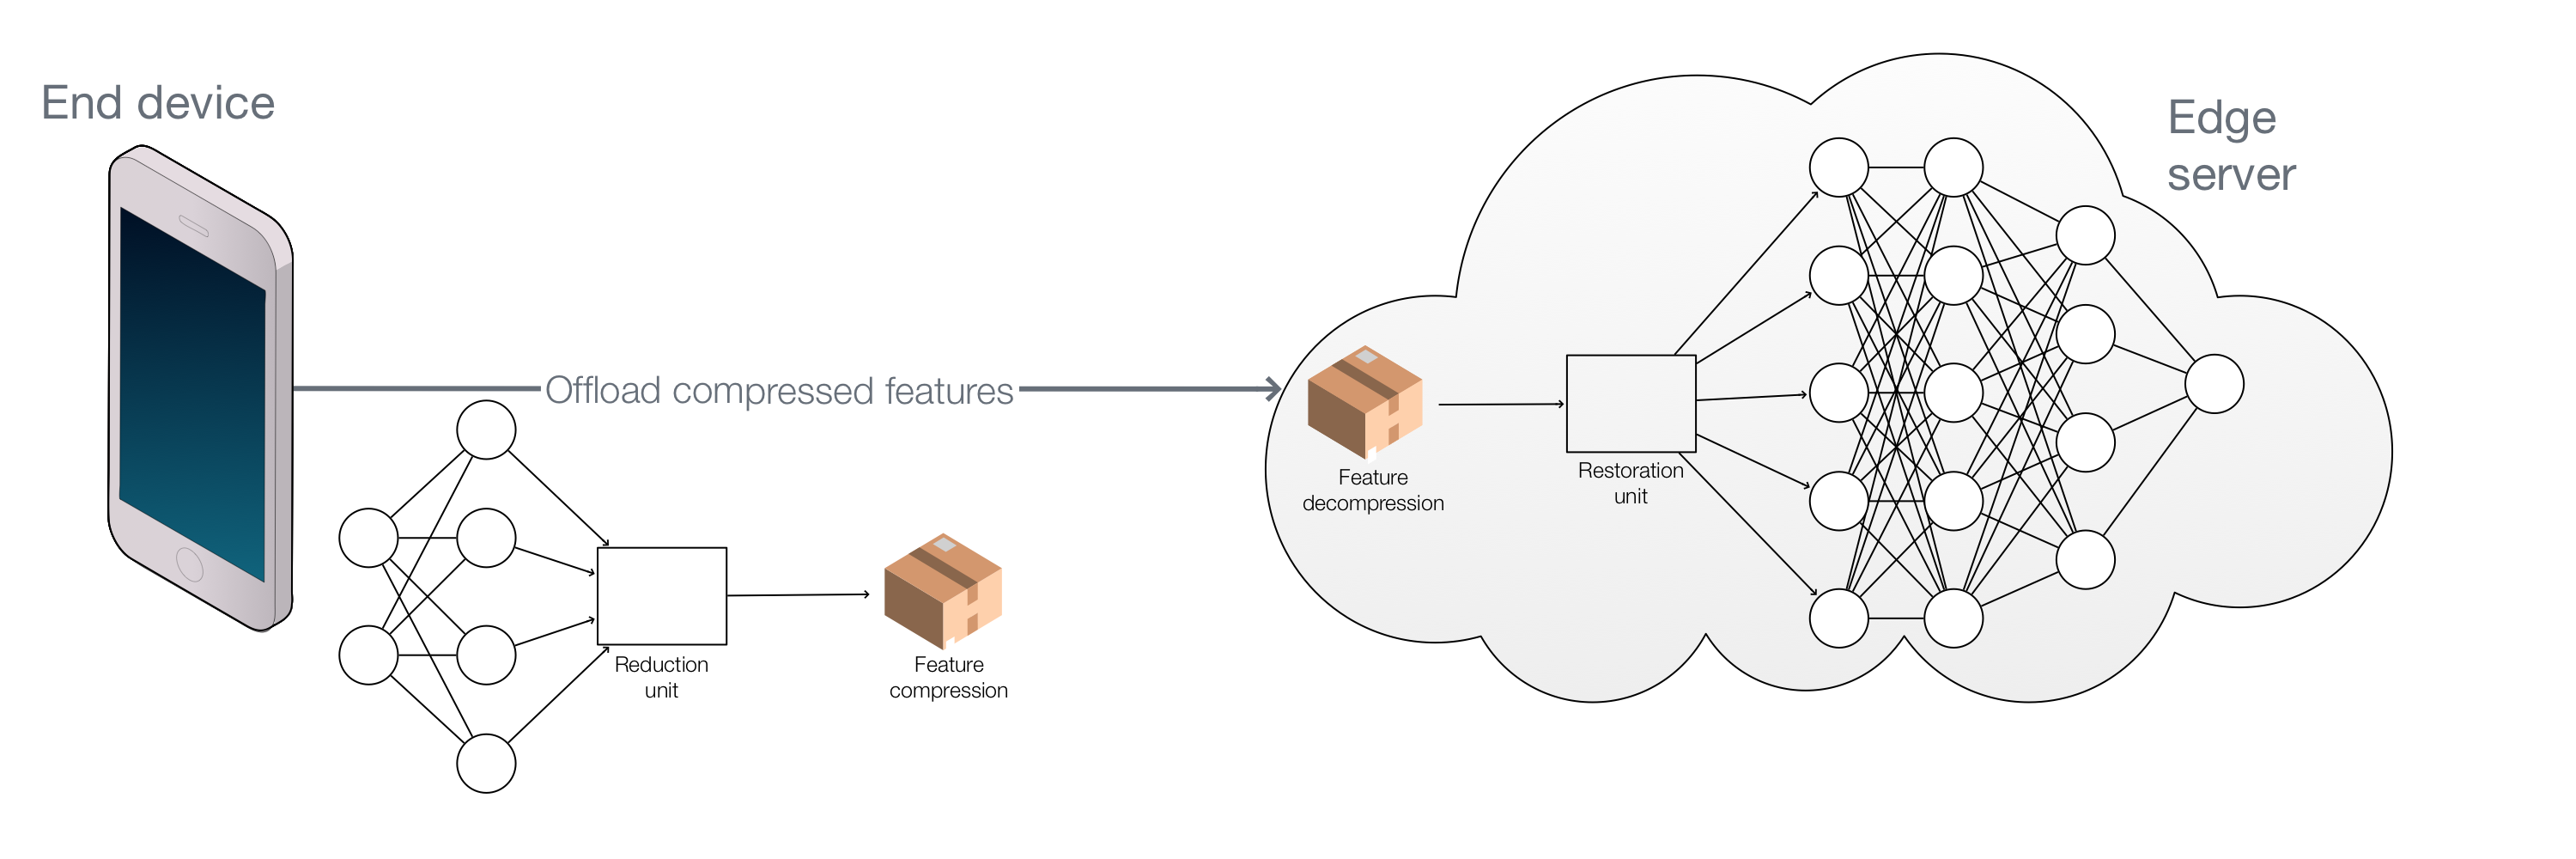
\includegraphics[width=\linewidth]{figures/models/bottlenet}
		\captionof{figure}[BottleNet Unit]{BottleNet Unit}
	\end{minipage}
	
	\gls{bottlenet} is able to achieve 84$\times$ bit savings compared to cloud-only approach with less than 2\% degradation of accuracy caused by lossy compression with compression-aware training. Under good networking condition, the evaluation of \gls{bottlenet} shows, that the best split is after the first convolutional block, as a smaller representation of the input can be found and the server is a more powerful machine. Compared to cloud-only approach using WiFi a 8$\times$ speed up is found. 
	
	\item[Collaborative Early Exit]
	
	Edgent \cite{li_edge_2018} is an optimization of the latency-accuracy trade-off for mission-critical application with a predefined deadline. It is built on top of the \gls{branchynet} model, and tries to handle the communication delay, by selecting an optimal exit and partitioning point to collaboratively process model inference on end device and edge. The optimization is based on a latency requirement, a regression model of inference time of each layer, and the observed available bandwidth between end device and edge server. Edgent is able to meet more stringent deadlines, than running solely \gls{branchynet} on device or edge. 
	
	Other approaches at distributing the early exit models takes advantage of the multiple exits, to locally terminate the process, if it is needless to use a later exit on edge or in cloud. Cascading neural network have been followed up in \cite{leroux_cascading_2017}. The paper uses the early exiting model, to distributes it between end devices, edge and cloud. Figure \ref{fig:early-exit-colab} illustrates a partitioned early exit \gls{dnn} for collaborative edge. 
	
	\begin{minipage}[t]{\linewidth}
		\centering
		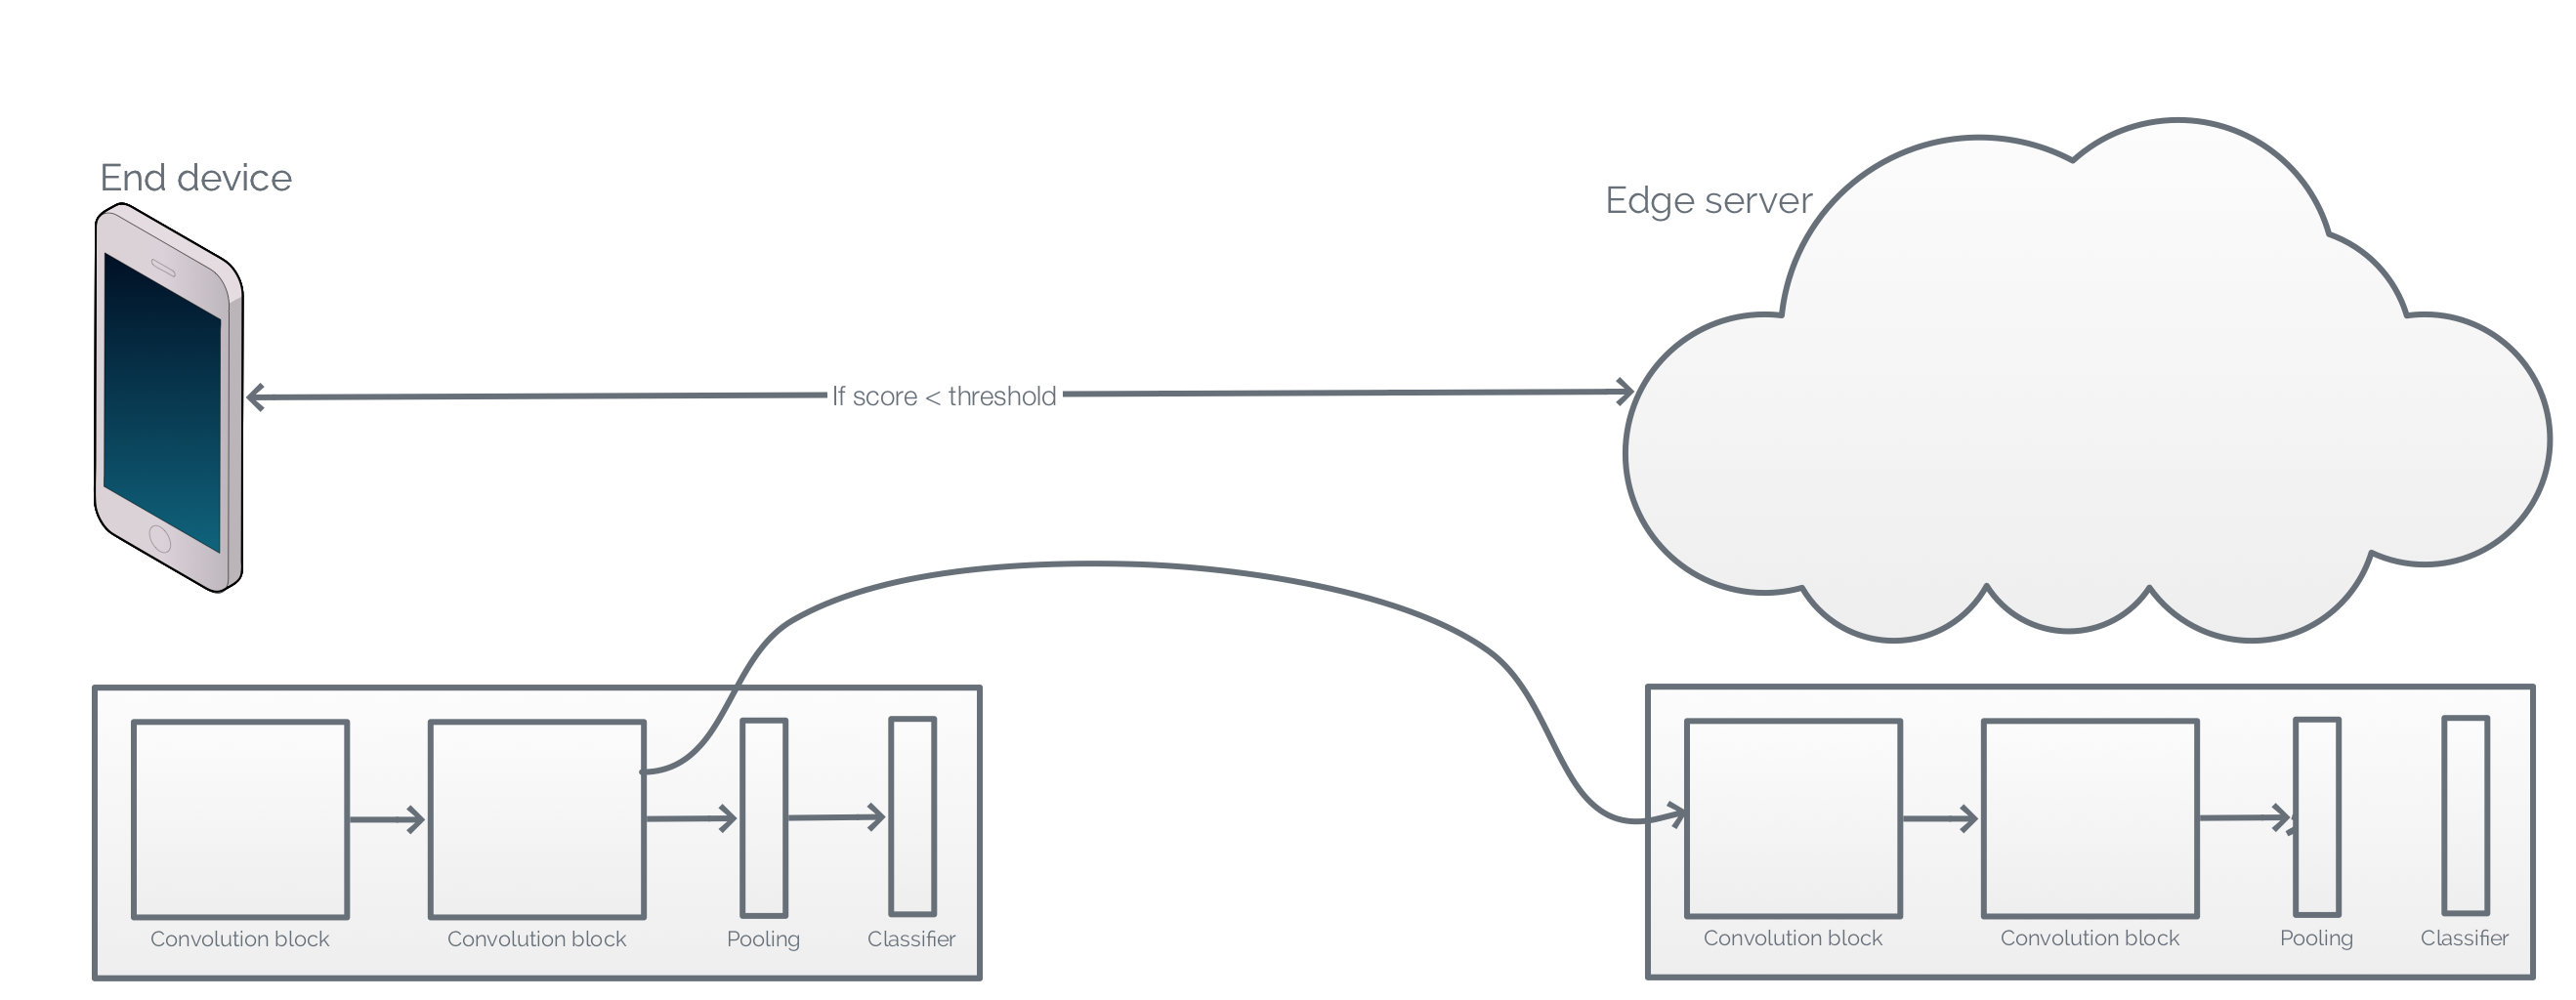
\includegraphics[width=\linewidth]{figures/models/cascaded}
		\captionof{figure}[Cascaded \gls{dnn} over a computing hierarchy]{Cascaded \gls{dnn} over a computing hierarchy}
		\label{fig:early-exit-colab}
	\end{minipage}

	The model is distributed in a manner, where one or more exits are processed by the end device, and one or more exits on the edge server. However, model partitioning introduces communication delay to the inference task, that most be accounted for e.g. using one of the method for model partitioning.
	
	\gls{ddnn} \cite{teerapittayanon_distributed_2017} extends the idea to formulate a framework, that allows for geographically distributed end devices to collaborative solve a \gls{dnn} inference task. The intermediate output from the geographically distributed end-devices are aggregated for a local prediction. Based on the score the inference is exited locally or sensor fusion of the intermediate features are performed by a \gls{dnn} at the edge and/or cloud. Using early exit model in this fashion, does not only show improvement for early exits but also the final prediction. Additionally \gls{ddnn} shows benefits from distributed computing to provide fault tolerance, when some local \gls{dnn} comes with a bad or missing prediction. \gls{ddnn} have been proposed for Industry 4.0 to solve autonomous defect detection in \cite{li_deep_2018}. 
\end{enumdescript}

\subsection{Distributed Inference}

Distributed inference is similar to collaborative edge. However, instead of partitioning the model in the depth axis i.e. between two layers, as for collaborative inference. Distributed inference seeks to partition the task in the input axis i.e. let multiple peers solve a single layers. \gls{modnn} \cite{mao_modnn:_2017} is a framework to distribute the computing of the input to multiple worker nodes. Distributing computation input-wise can result in a higher degree of data dependence, and lead to more a higher degree of communication between workers. \gls{modnn} show improvement of computing a \gls{dnn} inference on multiple mobile devices connected on a WLAN, compared to standalone inference on a single mobile device. DeepThings \cite{zhao_deepthings:_2018} is a framework intended for constraint \gls{iot} devices to distribute computation. In DeepThings, they take advantage of local region dependency in layers, that can be split into multiple tasks and that the dependency across layers into large tasks. In this manner, they actually split the network layers horizontally but stack the work vertically i.e. just as regularly \gls{dnn}s.









